\documentclass{tstextbook}

%\usepackage{rom}

\begin{document}

\newcommand{\myqq@}{'}
\catcode`\'=13
\newcommand{'}[1]{\ifmmode {}^\prime \noexpand#1%
 \else\ifx#1a\u{a}%
 \else\ifx#1i\^{\i}%
 \else\ifx#1s\c{s}%
 \else\ifx#1t\c{t}%
 \else\ifx#1A\u{A}%
 \else\ifx#1I\^{I}%
 \else\ifx#1S\c{S}%
 \else\ifx#1T\c{T}%
 \else\ifx#1"\myqq@%
   \fi\fi\fi\fi\fi\fi\fi\fi\fi%
 \fi}

\tsbook{Laborator de circuite electrice \break - concepte, simul'ari, experimente - \break\break
\break\break
{\small versiune din 4 martie 2020}}
       {Mihai Popescu, Ruxandra B'arbulescu, Sorin Lup, Gabriela Ciuprina, Daniel Ioan}
       {Cover Designer}
%       {3 iulie 2019}
       {xxxxx}{xxx--xx--xxxx--xx--x}{0.0}
       {}
%       {Iulie 2019}


%---------------------------------------------------------------------------
% Chapters
%---------------------------------------------------------------------------

%---------------------------------------------------------------------------
\chapter{Divizorul de tensiune}
\section{Introducere}

\begin{summary}
  Divizorul de tensiune se bazeaz'a pe distribuirea unei tensiuni $u$ 'intre componentele divizorului. Cel mai simplu exemplu 'in acest sens este un divizor de tensiune format din dou'a rezistoare conectate 'in serie (Fig. \ref{fig:divizor_schema_exemplu}), av\^and tensiunea \textit{de intrare} aplicat'a pe perechea de rezistoare 'si tensiunea \textit{de ie'sire} extras'a de pe una din componente ($u_1$ sau $u_2$). Divizorul rezistiv de tensiune este adesea folosit pentru a crea tensiuni de referin't'a, ca 'in Fig. \ref{fig:comparator_cu_divizor} sau pentru a reduce tensiunea provenit'a dintr-o re'tea complex'a.
\end{summary}

\begin{figure}[!b]
	\centering
		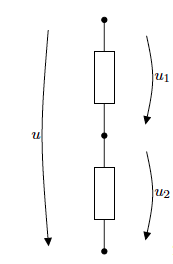
\includegraphics[width=0.19\textwidth]{laborator_01/figuri/divizor_schema_exemplu}
	\caption{Divizorul de tensiune.}
	\label{fig:divizor_schema_exemplu}
\end{figure}

\begin{figure}
	\centering
		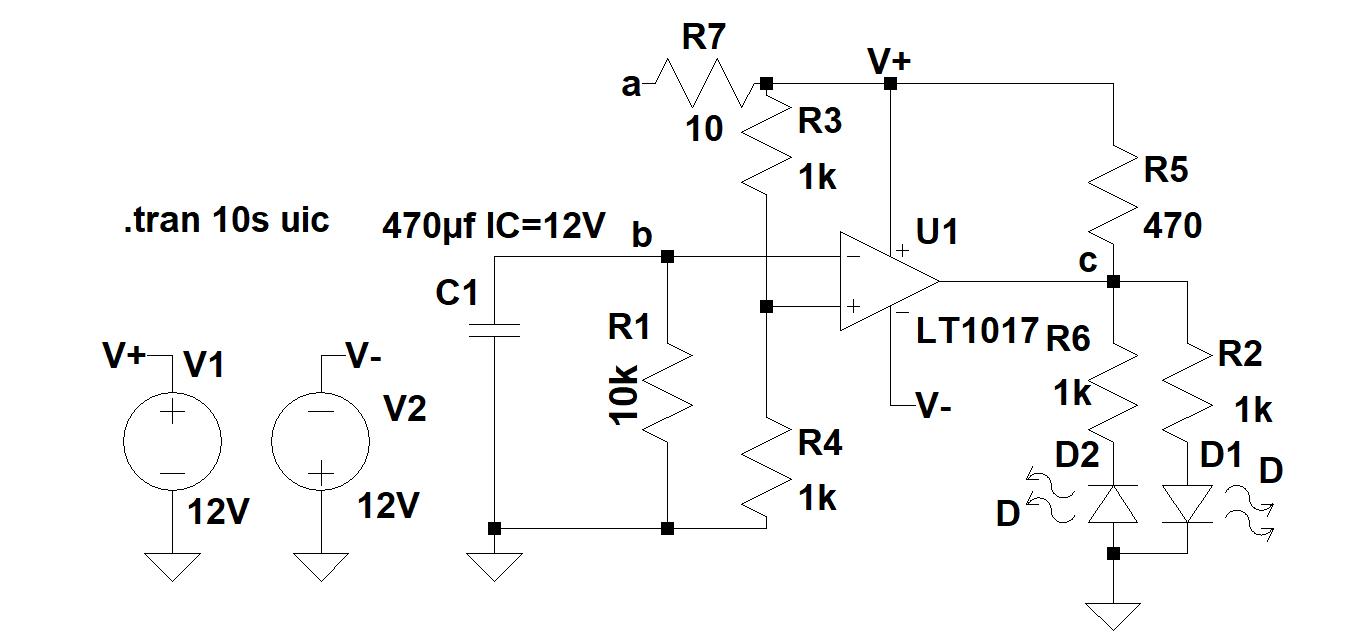
\includegraphics[width=0.8\textwidth]{laborator_01/figuri/comparator_cu_divizor}
	\caption{Circuit comparator cu tensiunea de referinta data de un divizor de tensiune format din $R_3$ 'si $R_4$.}
	\label{fig:comparator_cu_divizor}
\end{figure}

\subsection*{Scopul lucr'arii}

Obiectivul acestei lucr'ari de laborator este ilustrarea modului 'in care se 'imbin'a cele trei aspecte ale domeniului Calculelor stiintifice 'in inginerie (CSE -- \textit{Computational science and engineering}): conceptele (lumea ideilor), simul'arile (lumea virtuala) 'si experimentele (lumea real'a). 'In acest scop, exemplele folosite sunt simple din punct de vedere conceptual, tocmai pentru a permite nu numai explicarea aspectelor strict legate de teoria circuitelor, dar si eviden'tierea conexiunilor cu teoria sistemelor, metode numerice, analize pe baza simul'arilor 'in SPICE. Aceast'a lucrare de laborator creeaz'a o baz'a solid'a de analiz'a, astfel 'inc\^at trecerea la circuite mai complicate, cu elemente neliniare sau m'arimi variabile 'in timp s'a se fac'a relativ u'sor.

\subsection*{Concepte teoretice utile}

Pentru a putea efectua cu succes aceast'a lucrare trebuie s'a revede'ti urm'atoarele concepte prezentate la curs: intensitatea curentului electric, tensiunea electric'a, poten'tialul electric, legile lui Kirchhoff, rezistorul dipolar liniar, sursa ideal'a de tensiune. 
%Pentru a v'a verifica aceste cuno'stin'te completa'ti chestionarul 1 (vezi Anexa 1) de pe moodle.

%\begin{exercise}[Pe moodle, 'inainte de laborator]
%Efectua'ti chestionarul 1 de pe moodle. 'Incerca'ti s'a ob'tine'ti un punctaj c\^at mai mare.
%\end{exercise}


\section{Concepte}

\begin{summary}
  Aceast'a sec'tiune descrie conceptele necesare 'in'telegerii lucr'arii. Sunt analizate circuitele care vor fi studiate, prezent\^andu-se nu numai aspectele strict legate de teoria circuitelor, dar 'si conexiunile cu teoria sistemelor. Tot aici sunt explicate 'si concepte de metode numerice ce vor permite estimarea cantitativ'a a preciziei rezultatelor.  
\end{summary}

\subsection*{Circuitele studiate 'in aceast'a lucrare}

\subsubsection*{\color{blue} Divizorul de tensiune rezistiv 'in gol}

Figura \ref{fig:divizor_schema} prezint'a schema de principiu a unui divizor de tensiune rezistiv, 'in diferite variante de desenare. Tensiunea $U = V_+ - V_- = V_+|_{V_-=0}$ se aplic'a ansamblului de rezistoare conectate 'in serie, distribuindu-se 'in $U_1$ 'si $U_2=V_a - V_- = V_a|_{V_-=0}$.
\begin{figure}[h]
	\centering
		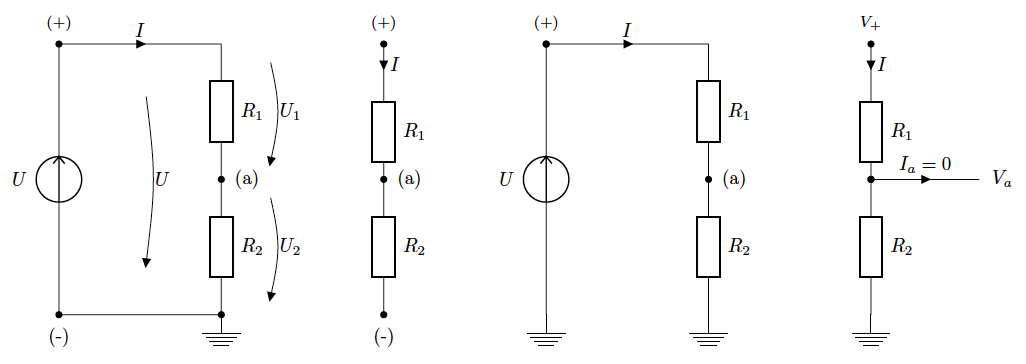
\includegraphics[width=0.75\textwidth]{laborator_01/figuri/scheme_divizor}
	\caption{Divizorul de tensiune -- schema de principiu 'in diferite variante de desenare.}
	\label{fig:divizor_schema}
\end{figure}

Cu nota'tiile din Fig. \ref{fig:divizor_schema} se demonstreaz'a u'sor c'a:
\begin{equation} \label{eq:tensiune_intrare_gol}
U_1 = \frac{R_1}{R_1+R_2}U
\end{equation}
\begin{equation} \label{eq:tensiune_iesire_gol}
U_2 = \frac{R_2}{R_1+R_2}U.
\end{equation}

\begin{exercise}%[Pe foaie de h\^artie, 'inainte de laborator]
Demonstra'ti rela'tiile (\ref{eq:tensiune_intrare_gol}) 'si (\ref{eq:tensiune_iesire_gol}).
\end{exercise}

\begin{retine}
  \label{retine1}
  \index{}
	Tensiunea pe fiecare rezistor al unui divizor de tensiune e propor'tional'a cu rezisten'ta rezistorului:
  \small
  \begin{equation*}
    \frac{U_1}{R_1} = \frac{U_2}{R_2}
  \end{equation*}
\end{retine}

Dac'a not'am cu $\alpha$ raportul dintre cele dou'a rezisten'te astfel:
\begin{equation}
\alpha = \frac{R_1}{R_2},
\end{equation}
atunci putem rescrie rela'tia (\ref{eq:tensiune_iesire_gol}) 'in func'tie de acest raport:
\begin{equation}
U_2 = \frac{1}{1+\alpha}U.
\end{equation}

Se spune c'a divizorul este cu ''$1+\alpha$''. Spunem c'a avem un \textit{divizor cu 3} dac'a valoarea numitorului este 3, deci raportul $\alpha = 2$, adic'a $R_1=2R_2$.

\begin{retine}
  \label{retine2}
  \index{}
%    Raportul dintre parametrii celor dou'a rezistoare influen'teaz'a raportul dintre tensiunea de ie'sire 'si tensiunea de intrare.
	Este util'a analiza urm'atoarelor cazuri particulare:
\begin{enumerate}
\item $R_1 = R_2 \Rightarrow \alpha = 1$, ''divizor cu 2''
\begin{equation*}
U_2 = \frac{U}{2}
\end{equation*}
\item $R_1 \gg R_2 \Rightarrow \alpha = 0$, ''divizor cu 1''
\begin{equation*}
U_2 \simeq U
\end{equation*}
\item $R_1 \ll R_2 \Rightarrow \alpha\rightarrow\infty$, ''divizor cu $\infty$''
\begin{equation*}
U_2 \simeq 0
\end{equation*}
\end{enumerate}
\end{retine}


\subsubsection*{\color{blue} Divizorul de tensiune rezistiv 'in sarcin'a} %\label{subsection:in_sarcina}

Divizorului de tensiune i se poate conecta o rezisten't'a de sarcin'a la ie'sire, 'in paralel cu $R_2$, a'sa cum este ar'atat 'in Figura \ref{fig:divizor_sarcina_schema}.

\begin{figure}[!b]
	\centering
		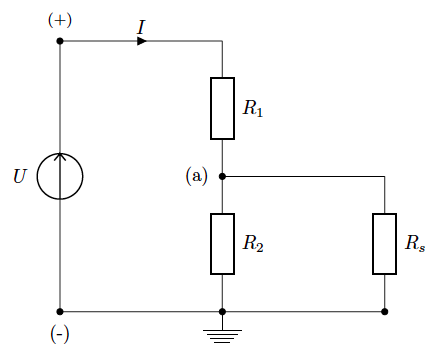
\includegraphics[width=0.5\textwidth]{laborator_01/figuri/scheme_divizor_sarcina}
	\caption{Divizorul de tensiune 'in sarcin'a -- schema de principiu.}
	\label{fig:divizor_sarcina_schema}
\end{figure}

'In acest caz, tensiunea de intrare se repartizeaz'a 'intre $R_1$ 'si grupul $R_2$ 'in paralel cu $R_s$. Rela'tia dintre tensiunea de ie'sire 'si cea de intrare devine:
\begin{equation} \label{eq:tensiune_iesire_sarcina}
U_2 = \frac{R_2\parallel R_s}{R_1+R_2\parallel R_s}U,
\end{equation}
unde $R_2\parallel R_s$ este o nota'tie pentru rezisten'ta echivalent'a a dou'a rezistoare conectate 'in paralel $R_2\parallel R_s = \frac{R_2R_s}{R_2+R_s}$.

Dac'a se dore'ste o tensiune de ie'sire aproximativ egal'a cu cea de la sec'tiunea precedent'a (ie'sire 'in gol), atunci rezisten'ta de sarcin'a $R_s$ trebuie aleas'a astfel 'inc\^at s'a fie mult mai mare dec\^at $R_2$ (de exemplu $R_s \approx 100R_2$), ceea ce ar determina ca $R_2\parallel R_s \approx R_2$:

\begin{equation}\label{eq:sarcina}
R_2 \parallel R_s = \frac{R_2 R_s}{R_2+R_s}\approx \frac{R_2 R_s}{R_s}=R_2, \text{ dac'a } R_s \gg R_2.
\end{equation}

\begin{retine}
Se poate crea un divizor cu $(1+\alpha)$ doar dac'a rezisten'ta de sarcin'a este suficient de mare.
\end{retine}

\subsubsection*{\color{blue} Puntea rezistiv'a} %\label{subsection:puntea_rezistiva}

Puntea rezistiv'a poate fi privit'a ca o extensie a divizorului de tensiune 'in gol, alc'atuit'a din dou'a divizoare de tensiune 'in  paralel. Grupul de rezistoare ($R_1$ 'in serie cu $R_2$) are 'in paralel o nou'a latur'a format'a din alte dou'a rezistoare conectate 'in serie ($R_3$ 'si $R_4$). Tensiunea de la bornele celor dou'a grupuri de rezistoare este aceea'si 'si egala cu $U=V_+$. Fiecare grup de rezistoare func'tioneaz'a ca un divizor de tensiune, astfel c'a putem extinde rela'tia (\ref{eq:tensiune_iesire_gol}) pentru tensiunile caracteristice pun'tii, notate cu $V_a$ 'si $V_b$:

\begin{figure}[!b]
	\centering
		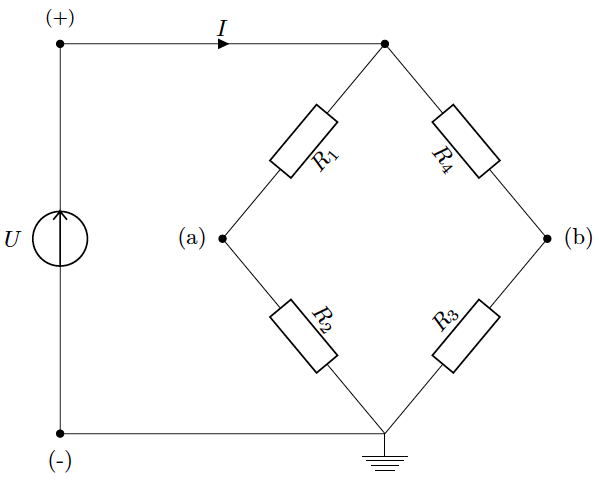
\includegraphics[width=0.5\textwidth]{laborator_01/figuri/scheme_punte_rezistiva}
	\caption{Puntea rezistiv'a -- schema de principiu. Tensiunea 'intre (a) 'si (b) este zero dac'a $R_1 R_3 = R_2 R_4$.}
	\label{fig:punte_rezistiva_schema}
\end{figure}

\begin{equation} \label{eq:tensiuni_punte_Va}
V_a = \frac{R_2}{R_1+R_2}U
\end{equation}
\begin{equation} \label{eq:tensiuni_punte_Vb}
V_b = \frac{R_3}{R_3+R_4}U.
\end{equation}

Puntea este \textit{'in echilibru} dac'a $V_a=V_b$, adic'a dac'a cele dou'a
divizoare au acela'si factor de divizare. Egal\^and rela'tiile (\ref{eq:tensiuni_punte_Va}) 'si (\ref{eq:tensiuni_punte_Vb}), reiese u'sor c'a pentru echilibru trebuie s'a avem rela'tia urm'atoare 'intre rezisten'te: $R_1 R_3 = R_2 R_4$.

\begin{exercise}%[pe foaie de h\^artie, 'inainte de laborator]
Ce se 'int\^ampl'a dac'a 'intre (a) 'si (b) se conecteaz'a o rezisten't'a $R_5$? Dar dac'a se face un scurt-circuit? Dar dac'a 'intre (a) 'si (b) se conecteaz'a o surs'a ideal'a de tensiune (SIT)?
\end{exercise}

\subsection*{Circuitele ca sisteme}\label{subsection:ca_sisteme}

Tensiunile 'si curen'tii dintr-un circuit reprezint'a \textit{semnale} 'in circuit, iar circuitul este un \textit{sistem} care r'aspunde la anumite semnale, produc\^and alte semnale.

Sursele din circuit furnizeaz'a \textit{excita'tiile} circuitului sau \textit{semnalele de intrare}, iar m'arimile de interes (tensiuni sau curen'ti) reprezint'a \textit{semnalele de ie'sire} sau \textit{r'aspunsurile}.

O reprezentare sistemic'a a divizorului de tensiune este 'in Fig. \ref{fig:divizor_tensiune_gol_sistem}.

\begin{figure}
	\centering
		
\includegraphics[width=0.5\textwidth]{laborator_01/figuri/divizor_tensiune_gol_sistem}
	\caption{Divizorul de tensiune ca sistem e caracterizat de $\alpha = \frac{R_1}{R_2}$.}
	\label{fig:divizor_tensiune_gol_sistem}
\end{figure}

Observa'ti c'a reprezentarea sistemic'a se face cu un ''bloc'' 'in care se v'ad semnalele de intrare (unul 'in acest caz) 'si semnalele de ie'sire (unul 'in acest caz, tensiunea $U_2$), iar pe figura care reprezint'a sistemul se marcheaz'a ''func'tia de transfer'', 'in cazul nostru o constant'a $H = \frac{1}{1+\alpha}$, astfel 'inc\^at $U_2 = HU$.

\begin{exercise}%[pe foaie de h\^artie, 'inainte de laborator]
  Realiza'ti o reprezentare sistemic'a a pun'tii rezistive.
\end{exercise}


\subsection*{Propagarea erorilor}

Componentele reale folosite 'in asamblarea circuitelor nu pot fi realizate perfect. Parametrii lor au anumite toleran'te, precizate de fabricant. De aceea, 'in proiectarea unui circuit, nu este important'a numai verificarea func'tion'arii dorite, ci 'si comportarea circuitului pe 'intreaga gam'a de varia'tie a parametrilor respectivi, impus'a de tehnologia de realizare a componentelor.

'In cazul exemplelor analizate 'in aceast'a lucrare, rezistoarele sunt realizate cu anumite toleran'te, marcate pe element (de exemplu 5\%, 10\%). Aceste toleran'te trebuie interpretate ca \textit{margini ale erorilor relative}.

Din aceast'a informa'tie putem deduce o margine a erorii absolute:
\begin{equation*}
\left|R_1-R_{1,\mathrm{nom}}\right| \leq r_1R_{1,\mathrm{nom}} \Longrightarrow a_1 = r_1R_{1,\mathrm{nom}}
\end{equation*}

\begin{retine}
  \label{retine3}
  \index{}
    Marginea erorii absolute se calculeaz'a ca fiind marginea erorii relative (toleran'ta) 'inmul'tit'a cu valoarea nominal'a. 
\end{retine}

Putem calcula acum intervalul de incertitudine 'in care se afl'a valoarea real'a a rezisten'tei:
\begin{align*}
\left|R_1-R_{1,\mathrm{nom}}\right| \leq a_1 \\
-a_1 \leq R_1 - R_{1,\mathrm{nom}} \leq a_1 \\
R_{1,\mathrm{nom}} - a_1 \leq R_1 \leq a_1 + R_{1,\mathrm{nom}} \\
R_1 \in [R_{1,\mathrm{nom}}-a_1, R_{1,\mathrm{nom}} + a_1] \\
\text{sau} \\
R_1 \in [R_{1,\mathrm{nom}}(1-r_1), R_{1,\mathrm{nom}}(1+r_1)]
\end{align*}

\begin{example}[]
  $R_1 = 2~\mathrm{k}\Omega \pm 5\%$ 'inseamn'a o valoare nominal'a $R_{1,\mathrm{nom}}=2~\mathrm{k}\Omega$ 'si o margine a erorii relative $r_1=5\%$, adic'a $\left|\frac{R_1-R_{1,\mathrm{nom}}}{R_{1,\mathrm{nom}}}\right| \leq r_1$.
 
  Marginea erorii absolute este:
   \begin{equation*}
    	a_1 = \frac{5}{100}\cdot 2 \cdot 10^3~\Omega = 100~\Omega = 0.1~\mathrm{k}\Omega
  \end{equation*}
  Deci valoarea real'a $R_1 \in [1.9, 2.1]~\mathrm{k\Omega}$.
\end{example}

\begin{retine}
  \label{retine4}
  \index{}
    Toate componentele au toleran'te de fabrica'tie! Ce leg'atur'a crede'ti c'a exist'a 'intre pre'tul unei componente 'si toleran'ta ei?
\end{retine}

Pentru a putea estima efectul acestor toleran'te asupra rezultatelor trebuie s'a folosim teorema de propagare a erorilor. \footnote{Aceste teoreme le ve'ti studia sau le-a'ti studiat deja la disciplina Metode numerice}.

S'a presupunem c'a o anumit'a marime $y$ (rezultat) depinde de $p$ parametri (date de intrare) independen'ti:
\begin{equation*}
y = f(x_1, x_2, ..., x_p).
\end{equation*}

Perturba'tia absolut'a a rezultatului $\Delta y$ se poate aproxima 'in func'tie de perturba'tiile absolute ale datelor de intrare ca:
\begin{equation*} \label{eq:deltay}
\Delta y \simeq \frac{\partial f}{\partial x_1}\Delta x_1 + \frac{\partial f}{\partial x_2}\Delta x_2 + ... + \frac{\partial f}{\partial x_p}\Delta x_p.
\end{equation*}

De unde:
\begin{align*}
\left|\Delta y \right| 
&\leq 
\left|\frac{\partial f}{\partial x_1}\right|\left|\Delta x_1\right| + \left|\frac{\partial f}{\partial x_2}\right|\left|\Delta x_2\right| + ... + \left|\frac{\partial f}{\partial x_p}\right|\left|\Delta x_p\right| \\
&\leq 
\left|\frac{\partial f}{\partial x_1}\right| a_{x_1} + \left|\frac{\partial f}{\partial x_2}\right| a_{x_2} + ... + \left|\frac{\partial f}{\partial x_p}\right| a_{x_p}.
\end{align*}

Marginea erorii absolute a rezultatului este 'in consecin't'a:
\begin{equation} \label{eq:margine_err_abs}
a_y = \left|\frac{\partial f}{\partial x_1}\right| a_{x_1} + \left|\frac{\partial f}{\partial x_2}\right| a_{x_2} + ... + \left|\frac{\partial f}{\partial x_p}\right| a_{x_p}.
\end{equation}

\begin{example}[]
  Adunarea a dou'a numere $x_1, x_2 > 0$ sau $x_1, x_2 < 0$:
  \begin{align*}
    y = x_1 + x_2, \\
    f(x_1,x_2) = x_1 + x_2
  \end{align*}

Din aplicarea (\ref{eq:margine_err_abs}) rezult'a:
\begin{equation} 
a_y = a_{x_1} + a_{x_2},~\text{deoarece} \left|\frac{\partial f}{\partial x_1}\right| = \left|\frac{\partial f}{\partial x_2}\right| = 1.
\end{equation}
\end{example}
\begin{example}[]
Sc'aderea a dou'a numere $x_1, x_2 > 0$ sau $x_1, x_2 < 0$:
  \begin{equation*}
    y = x_1 - x_2,\\
    f(x_1,x_2) = x_1 - x_2,
  \end{equation*}
  atunci din \ref{eq:margine_err_abs}
\begin{equation} 
a_y = a_{x_1} + a_{x_2},~\text{deoarece} \left|\frac{\partial f}{\partial x_1}\right| = \left|\frac{\partial f}{\partial x_2}\right| = 1.
\end{equation}
\end{example}

\begin{definition}[]
  Cum se analizeaz'a erorile relative? \\
  Din (\ref{eq:deltay}) rezult'a c'a 
  \begin{align*}
    &\frac{\Delta y}{y} \simeq \frac{1}{f}\frac{\partial f}{\partial x_1}\Delta x_1 + \frac{1}{f}\frac{\partial f}{\partial x_2}\Delta x_2 + ... + \frac{1}{f}\frac{\partial f}{\partial x_p}\Delta x_p \\
    \Longrightarrow 
    &\frac{\Delta y}{y} \simeq \frac{x_1}{f}\frac{\partial f}{\partial x_1}\frac{\Delta x_1}{x_1} + \frac{x_2}{f}\frac{\partial f}{\partial x_2}\frac{\Delta x_2}{x_2} + ... + \frac{x_p}{f}\frac{\partial f}{\partial x_p}\frac{\Delta x_p}{x_p} \\
    \Longrightarrow 
    \left|\frac{\Delta y}{y}\right| &\leq \left|\frac{x_1}{f}\frac{\partial f}{\partial x_1}\right|\left|\frac{\Delta x_1}{x_1}\right| + \left|\frac{x_2}{f}\frac{\partial f}{\partial x_2}\right|\left|\frac{\Delta x_2}{x_2}\right| + ... + \left|\frac{x_p}{f}\frac{\partial f}{\partial x_p}\right|\left|\frac{\Delta x_p}{x_p}\right|\\
    &\leq \left|\frac{x_1}{f}\frac{\partial f}{\partial x_1}\right| r_{x_1} + \left|\frac{x_2}{f}\frac{\partial f}{\partial x_2}\right| r_{x_2} + ... + \left|\frac{x_p}{f}\frac{\partial f}{\partial x_p}\right| r_{x_p}.\\
  \end{align*}
\end{definition}

Marginea erorii relative a rezultatului este:
\begin{equation} \label{eq:margine_err_rel}
r_y = \left|\frac{x_1}{f}\frac{\partial f}{\partial x_1}\right| r_{x_1} + \left|\frac{x_2}{f}\frac{\partial f}{\partial x_2}\right| r_{x_2} + ... + \left|\frac{x_p}{f}\frac{\partial f}{\partial x_p}\right| r_{x_p}.
\end{equation}

\begin{example}[]
  'Inmul'tirea a dou'a numere $x_1, x_2$:
  \begin{align*}
    y = x_1 x_2, \\
    f(x_1,x_2) = x_1 x_2
  \end{align*}

Din aplicarea (\ref{eq:margine_err_rel}) rezult'a:
\begin{equation} 
r_y = r_{x_1} + r_{x_2}.
\end{equation}

Similar, la 'imp'ar'tirea $y=\frac{x_1}{x_2}$ rezult'a $r_y = r_{x_1} + r_{x_2}$.
\end{example}

\begin{retine}
  \label{retine5}
  \index{}\textcolor{black!5}{!}
    \begin{enumerate}
      \item La adunare 'si sc'adere marginile erorilor \textbf{absolute} se adun'a.
      \item La 'inmul'tire 'si 'imp'ar'tire marginile erorilor \textbf{relative} se adun'a.
    \end{enumerate}
\end{retine}

\begin{figure}
	\centering
		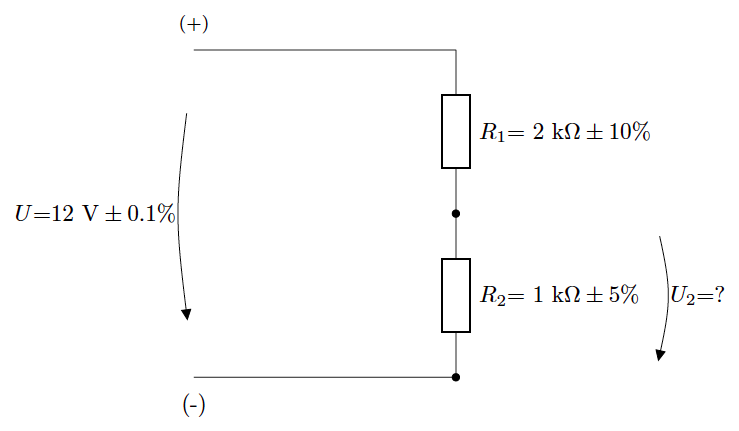
\includegraphics[width=0.6\textwidth]{laborator_01/figuri/exemplu_erori}
	\caption{Divizor de tensiune, elemente cu toleran'te.}
	 \label{fig:exemplu_erori}
\end{figure}

\begin{example}[]
  Fie divizorul de tensiune 'in care datele au toleran'tele marcate pe Fig.~\ref{fig:exemplu_erori}.
%
S'a calcul'am
\begin{equation} \label{eq:exemplu_erori}
U_2 = \frac{R_2}{R_1+R_2}U,
\end{equation}
valoarea nominal'a 'si eroarea ei, aplic\^and cele dou'a reguli de mai sus.

Vom efectua calculele 'in urm'atoarea ordine:
\begin{enumerate}
\item Adunarea $R_1+R_2$
\item 'Imp'ar'tirea dintre $R_2$ 'si rezultatul adun'arii de la punctul 1.
\item 'Inmul'tirea dintre $U$ 'si rezultatul de la 2.
\end{enumerate}

S'a le lu'am pe r\^and:
\begin{enumerate}
\item \textcolor{Bittersweet}{$R_1 = 2~\mathrm{k}\Omega\pm10\%, R_2 = 1~\mathrm{k}\Omega\pm5\% \Longrightarrow R_1+R_2=?$}\\
Valoarea nominal'a $R_1 + R_2 = 3~\mathrm{k}\Omega$.
  \begin{align*}
    a_{R_1} = e_{R_1}R_1 = \frac{10}{100}\cdot 2~\mathrm{k}\Omega = 0.2~\mathrm{k}\Omega \\
    a_{R_2} = e_{R_2}R_2 = \frac{5}{100}\cdot 1~\mathrm{k}\Omega = 0.05~\mathrm{k}\Omega \\
    \Longrightarrow a_{R_1+R_2} = a_{R_1} + a_{R_2} = 0.25 ~K\Omega.
  \end{align*}
La adunare 'stim c'a marginile erorilor absolute se adun'a. De aceea e necesar s'a calcul'am mai 'int\^ai aceste margini:

Eroarea relativa 
\begin{equation*}
r_{R_1+R_2} = \frac{a_{R_1+R_2}}{R_1+R_2} = \frac{0.25~\mathrm{k}\Omega}{3~\mathrm{k}\Omega} = \frac{0.25}{3} = \frac{25}{3}\% \simeq 8.4\%
\end{equation*}

\item \textcolor{Bittersweet}{$R_2 = 1~\mathrm{k}\Omega\pm5\%, R_1+R_2 = 3~\mathrm{k}\Omega\pm8.4\% \Longrightarrow \frac{R_2}{R_1+R_2}=?$}

La 'imp'ar'tire marginile erorilor relative se adun'a, deci:
\begin{equation*}
\frac{R_2}{R_1+R_2} = \frac{1}{3} \pm 13.4\%
\end{equation*}


\item \textcolor{Bittersweet}{$\frac{R_2}{R_1+R_2} = \frac{1}{3} \pm 13.4\%, U=12~\mathrm{V}\pm0.1\% \Longrightarrow U_2 = \frac{R_2}{R_1+R_2}U=?$}

La 'inmul'tire marginile erorilor relative se adun'a.

Deci $U_2 = \frac{1}{3}12~\mathrm{V} \pm 13.5\% = 4~\mathrm{V} \pm 13.5\%$.

Acest lucru 'inseamn'a de fapt c'a 
\begin{align*}
U_2 &\in \left[4\left(1-\frac{13.5}{100}\right), 4\left(1+\frac{13.5}{100}\right)\right]~\mathrm{V} \\
U_2 &\in \left[3.46, 4.54\right]~\mathrm{V}.
\end{align*}
\end{enumerate}
\end{example}

'In preg'atirea laboratorului, v'a recomand'am ca toate aceste calcule s'a le face'ti 'intr-o foaie de calcul organizat'a ca 'in Fig. \ref{fig:divizor_tensiune_excel1}.

\begin{figure}
	\centering
		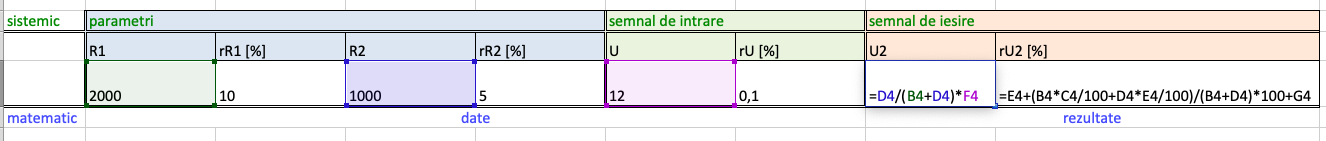
\includegraphics[width=1\textwidth]{laborator_01/figuri/divizor_tensiune_excel1}
	\caption{Divizor de tensiune 'in gol, foaie de calcul cu m'arimi calculate.}
	 \label{fig:divizor_tensiune_excel1}
\end{figure}

\begin{exercise}%[fi'sier .xls, 'inainte de laborator]
  Relua'ti ra'tionamentul de mai sus 'si completa'ti o foaie de calcul 'in care s'a evalua'ti semnalul de ie'sire $U_2$ pentru un divizor de tensiune 'in sarcin'a, consider\^and urm'atoarele toleran'te pentru parametri 'si semnalul de intrare: $R_1 = 2~\Omega\pm5\%$, $R_2 = 4~\Omega\pm10\%$, $R_s = 4~\mathrm{k}\Omega\pm10\%$, $U = 18~V\pm0.5\%$.
\end{exercise}
\begin{exercise}%[fi'sier .xls, 'inainte de laborator]
  Relua'ti ra'tionamentul de mai sus pentru calculul $V_a-V_b$ pentru o punte rezistiv'a, unde valorile nominale ale rezistoarelor sunt: $R_1 = 2~\Omega$, $R_2 = 6~\Omega$, $R_3 = 9~\Omega$, $R_4 = 3~\Omega$, toate rezistoarele au toleran'ta $5\%$, iar $U = 20~\mathrm{V}\pm0.1\%$.
\end{exercise}

\subsection*{Chestionar preliminar:  Concepte}

%Pentru a verifica 'in'telegerea conceptelor descrise 'in acest capitol, rula'ti chestionarul 2 (vezi Anexa 2) de pe moodle.

\begin{exercise}%[Pe moodle, 'inainte de laborator]
Efectua'ti chestionarul de antrenament de pe moodle ("Concepte").
\end{exercise}
\section{Simul'ari}
\label{sec:ltspice}
\subsection*{LTSpice}


LTSpice este un simulator de circuite, 'in care circuitele pot fi descrise ca un fi'sier text cu o list'a de elemente, numit \textit{netlist} sau ca o schema de circuit (desen), numit'a \textit{schematics} \cite{ltspice}. Este util'a 'in'telegerea modului de lucru 'in ambele variante, avantajele 'si dezavantajele lor.

 \begin{itemize}
 \item[--] Lucrul cu \textit{netlist} are avantajul c'a fi'sierul generat este portabil ('in propor'tie destul de mare) 'intre diferitele simulatoare de circuite (PSpice, LTSpice, ngspice, etc.). Dac'a schema este foarte complicat'a, lucrul cu acest fi'sier devine greoi, eventualele gre'seli fiind greu de depistat. 'In plus, este necesar'a cunoa'sterea precis'a a sintaxei. 
 \begin{example}[Fi'sier netlist corespunz'ator circuitului din Fig. \ref{fig:comparator_cu_divizor}]
\textcolor{white}{!}\\
\textcolor{OliveGreen}{* circuit comparator cu tensiunea de referinta}\\
\textcolor{OliveGreen}{* data de un divizor de tensiune}\\
R1 b 0 10k \\
C1 b 0 470uf IC=12V \\
R3 V+ N001 1k \\
R4 N001 0 1k \\
XU1 N001 b V+ V- c LT1017 \\
R2 P001 c 1k \\
D1 P001 0 D \\
D2 0 P002 D \\
R5 V+ c 470 \\
R6 c P002 1k \\
R7 V+ a 10\\
V1 V+ 0 12V\\ 
V2 0 V- 12V \\
%\textcolor{blue}{.model D D /Library/Application Support/LTspice/lib/cmp/standard.dio }\\
\textcolor{blue}{.tran 10s uic} \\
%\textcolor{blue}{.lib LTC1.lib}\\
%\textcolor{blue}{.backanno}\\
\textcolor{blue}{.end}\\
\end{example} 

\item[--] Lucrul cu \textit{schematics} are avantajul c'a este intuitiv. Dezavantajul provine din faptul c'a fi'sierul generat nu este portabil 'intre diferite simulatoare. Dac'a se dore'ste 'ins'a migrarea c'atre un alt simulator, atunci se poate exporta netlistul asociat. Un alt dezavantaj este acela c'a, 'in cazul elementelor nepolarizate (de ex. rezistoarele), utilizatorul nu are un control imediat al sensului de referin't'a al laturii. Pentru a 'in'telege acest sens de referin't'a trebuie inspectat netlistul.
 \end{itemize} 
 
\subsection*{Hands-on it!}

Vom exemplifica generarea unui netlist pentru un divizor de tensiune rezistiv, 'in gol, format din dou'a rezistoare $R_1 = 360~\Omega$ 'si $R_2 = 180~\Omega$, la bornele c'aruia se aplic'a o tensiune de 6 V, ca in Fig. \ref{fig:spice_ex1_1_2} st\^anga. 

\begin{figure}
	\centering
		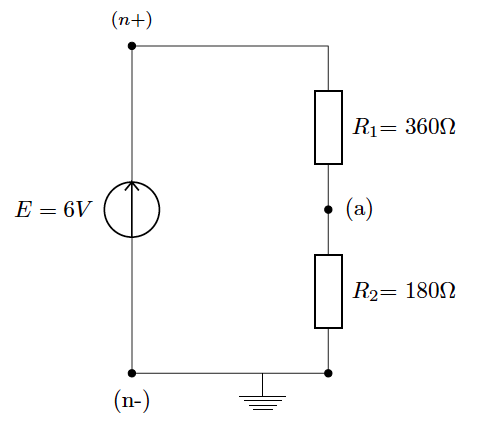
\includegraphics[width=0.5\textwidth]{laborator_01/figuri/spice_divizor_gol_ex1}
		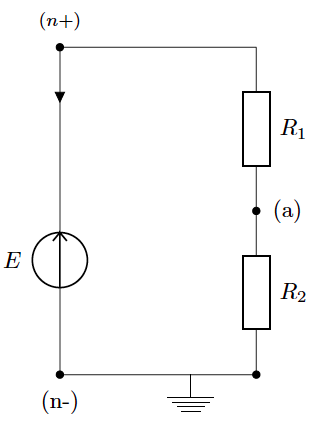
\includegraphics[width=0.33\textwidth]{laborator_01/figuri/spice_divizor_gol_ex1_crt}
	\caption{Divizor de tensiune 'in gol, exemplu. St\^anga: circuit cu noduri etichetate, dreapta: sens curent pentru SIT.}
	\label{fig:spice_ex1_1_2}
\end{figure}

Pentru crearea netlistului, circuitul trebuie preg'atit astfel:
\begin{enumerate}
\item Se pun noduri la bornele tuturor elementelor de circuit.
\item Se alege un nod la mas'a 'si se eticheteaz'a nodurile. Eticheta nodului de mas'a va fi obligatoriu 0.
\item Se aleg sensuri de referin't'a pentru curen'ti. Fiecare latur'a devine orientat'a, de la un nod ini'tial la un nod final.

\begin{retine}
  \label{retine3_1}
  \index{}
    'In cazul surselor ideale de tensiune este obligatorie reprezentarea sensului de referin't'a al curentului 'in sens opus sensului tensiunii electromotoare (ca 'in Fig. \ref{fig:spice_ex1_1_2} dreapta).
\end{retine}

%\begin{figure}
%	\centering
%		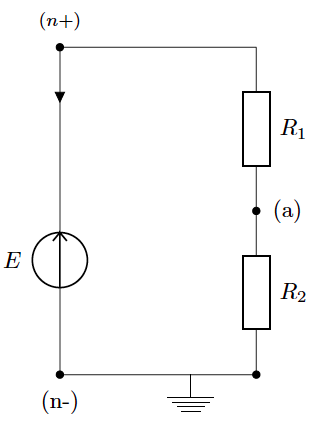
\includegraphics[width=0.3\textwidth]{laborator_01/figuri/spice_divizor_gol_ex1_crt}
%	\caption{Divizor de tensiune 'in gol -- sens curent pentru SIT.}
%	\label{fig:spice_ex1_2}
%\end{figure}

\item Se scrie fi'sierul netlist (numit de ex. divizorTensiuneGol.cir): \\
\textcolor{OliveGreen}{* Divizorul de tensiune} \\
\textcolor{OliveGreen}{* in gol}

\begin{figure}[!b]
	\centering
		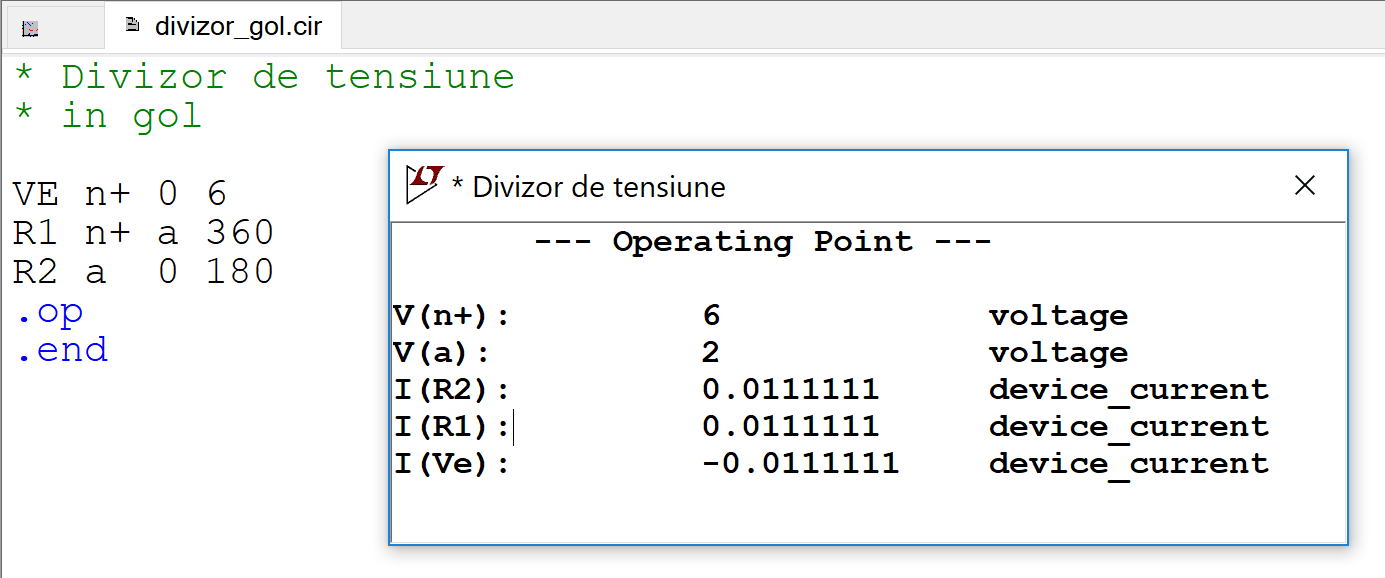
\includegraphics[width=0.7\textwidth]{laborator_01/figuri/spice_divizor_gol_op}
	\caption{Divizor de tensiune 'in gol -- rezultatul simul'arii.}
	\label{fig:spice_ex1_3}
\end{figure}
\begin{figure}[!b]
	\centering
		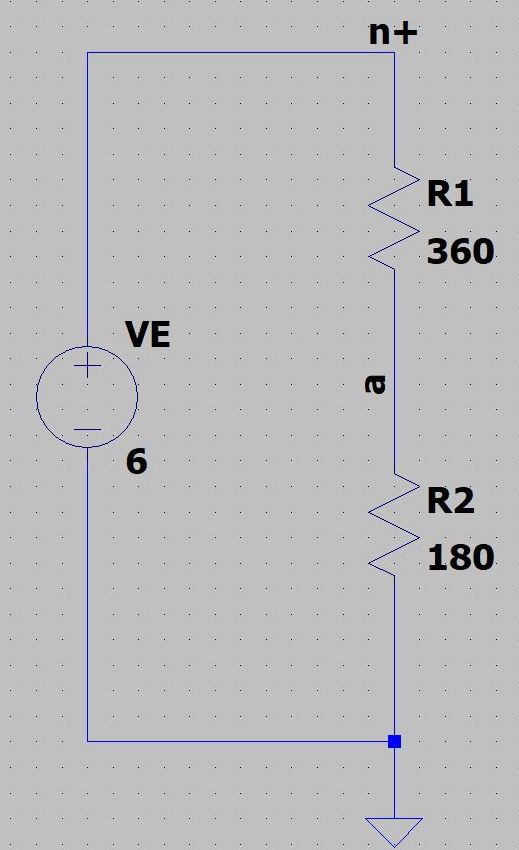
\includegraphics[width=0.33\textwidth]{laborator_01/figuri/spice_divizor_schematics}
	\caption{Divizor de tensiune 'in gol -- circuitul 'in \textit{schematics}.}
	\label{fig:spice_ex1_4}
\end{figure}

VE n+ 0 6 \\
R1 n+ a 360 \\
R2 a  0 180 \\
\textcolor{blue}{.op} \\
\textcolor{blue}{.end} 

\begin{itemize}
\item[--] Liniile care 'incep cu * reprezint'a comentarii.
\item[--] Prima linie din fi'sier este intotdeauna interpretat'a ca un comentariu.
\item[--] Fiecare linie reprezint'a o latur'a (un element).
\item[--] Primul caracter al unei linii indic'a tipul elementului (de ex. V pentru SIT, R pentru rezistor).
\item[--] Sintaxa liniei de tip SIT este:

$\mathrm{V_{nume}~~n+~~n-~~valoare}$

unde \textit{n+} reprezint'a nodul ini'tial al laturii, \textit{n-} reprezint'a nodul final, iar \textit{valoare} reprezint'a tensiunea electromotoare.
\item[--] Sintaxa liniei de tip R este:

$\mathrm{R_{nume}~~n+~~n-~~valoare}$

unde \textit{n+} reprezint'a nodul ini'tial al laturii, \textit{n-} reprezint'a nodul final, iar \textit{valoare} reprezint'a rezisten'ta. 
\item[--] Nodul de mas'a are intotdeauna eticheta 0 'si trebuie s'a existe 'in circuit.
\item[--] Liniile care 'incep cu . reprezint'a directive SPICE. 'In cazul exemplului studiat, \textit{.op} este o directiv'a de simulare 'in c.c. (o.p. = \textit{operational point} = \textit{punct static de func'tionare})
\item[--] Liniile de dup'a \textit{.end} sunt ignorate.

\end{itemize}
\end{enumerate}

Rezultatul simul'arii acestui netlist este Fig. \ref{fig:spice_ex1_3}. Observa'ti c'a $V_a = 2~\mathrm{V}$, a'sa cum era as'teptat, divizorul fiind cu 3.

\begin{figure}
	\centering
		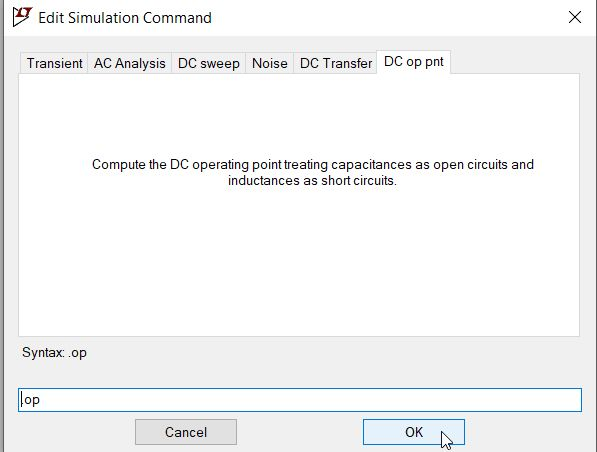
\includegraphics[width=0.45\textwidth]{laborator_01/figuri/spice_divizor_comanda_simulare}
	\caption{Divizor de tensiune 'in gol -- fereastr'a de stabilire a tipului de simulare.}
	\label{fig:spice_ex1_5}
\end{figure}

Generarea schemei se poate face 'si printr-o interfa't'a grafic'a (Fig. \ref{fig:spice_ex1_4}). Rularea se face apasand pe butonul Run 
\includegraphics[width=0.03\textwidth]{laborator_01/figuri/spice_Run_icon}. Dac'a a fost omis'a comanda de simulare, atunci programul conduce automat c'atre o fereastr'a de unde se stabile'ste tipul de simulare (Fig. \ref{fig:spice_ex1_5}).

'In {\em schematics}, etichetarea unui nod se face din Meniul \textbf{Edit $\rightarrow$ Label Net} sau direct cu \textbf{F4}, iar generarea fi'sierului netlist se face din meniul \textbf{View $\rightarrow$ SPICE Netlist}. Netlist-ul poate fi salvat ca fi'sier separat pentru modific'ari ulterioare cu click-dreapta 'in fereastr'a 'si alegerea \textbf{Edit as Independent netlist}.

Mai multe detalii despre SPICE se g'asesc 'in \cite{ltspice} 'si \cite{ltspicewiki}.

\begin{definition}[facultativ] Toleran'te 'in Spice\\
LTSpice permite descrierea elementelor cu toleran'te, una dintre metode fiind analiza Monte Carlo (Fig. \ref{fig:spice_tolerante}). Se definesc trei parametri care reprezint'a toleran'tele pentru $R_1$, $R_2$ 'si $U$. Valorile celor trei m'arimi sunt 'inlocuite cu un model Monte Carlo, care pentru sintaxa $mc(val,tol)$ variaz'a valoarea $val$ aleatoriu conform unei distribu'tii uniforme 'intre $val(1+tol)$ 'si $val(1-tol)$. 'In concluzie, aceste valori reprezint'a marginile erorilor relative ale elementelor (toleran'tele).\\

Vom considera c'a rezistoarele au toleran'ta 5\%, iar tensiunea de alimentare $U$ are marginea erorii absolute egal'a cu $0.1$ V. Remarca'ti c'a de aceast'a dat'a este dat'a eroarea absolut'a pentru tensiunea de intrare, nu cea relativ'a ca p\^an'a acum. Toleran'tele definite in Spice sunt relative, deci trebuie calculat'a marginea erorii relative pentru $U$, care este:
\begin{equation*} 
r_U = \frac{a_U}{U} = 0.0167 = 1.67\%.
\end{equation*}

Directiva:\\
.step param run 1 500 1 \\
arat'a c'a se vor executa 500 de simul'ari, fiecare simulare folosind pentru valori diferite ale elementelor. 

Forma general'a a acestei directive SPICE este: \\
.step param \textless nume parametru\textgreater \textless start\textgreater \textless stop\textgreater \textless pas\textgreater\\

Dac'a din Fig. \ref{fig:spice_tolerante} alegem valoarea minim'a 'si valoarea maxim'a pentru tensiunea de ie'sire $U_2 = V_a$, putem calcula marginea erorii relative care nu ar trebui s'a dep'a'seasc'a valoarea calculat'a de 11.7\%.
Pentru exemplul considerat, valoarea $U_2 = V_a \in [1.861, 2.1326], V_a \in \left[2-6.91\%, 2+6.63\%\right]$.\\

Putem analiza 'in Spice 'si cazul cel mai defavorabil (\textit{worst-case scenario}), 'in care datele au valorile minime 'si maxime. Pentru acest lucru 'inlocuim modelul Monte Carlo cu o func'tie proprie, care pentru prima execu'tie 'intoarce valorile nominale, iar pentru urm'atoarele execu'tii 'intoarce aleatoriu valorile minime sau maxime pentru cele trei m'arimi (func'tia \textit{flat} 'intoarce un num'ar aleatoriu 'intre -1 'si 1).\\

Fig. \ref{fig:spice_tolerante_wc} con'tine schema 'si rezultatele pentru 50 de simulari de acest tip. Valorile tensiunii de ie'sire sunt 'in intervalul $[1.8365, 2.17]$, ceea ce corespunde unei erori relative de $V_a \in \left[2-6.95\%, 2+7.325\%\right]$.
\end{definition} 

\begin{figure}[h]
	\centering
		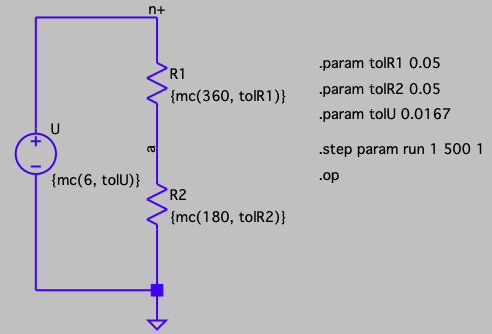
\includegraphics[width=0.42\textwidth]{laborator_01/figuri/spice_schematics_tolerante}
		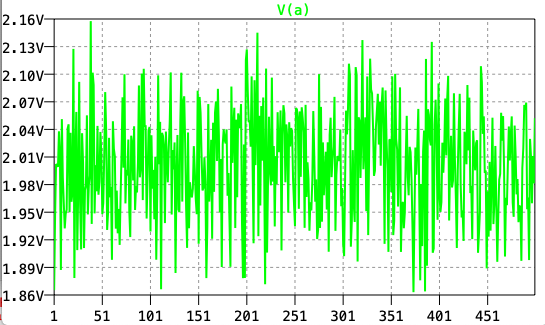
\includegraphics[width=0.5\textwidth]{laborator_01/figuri/spice_rezultate_tolerante}
	\caption{Divizor de tensiune 'in gol -- m'arimi cu toleran'te, {\em schematics} 'si rezultate.}
	\label{fig:spice_tolerante}
%\end{figure}
%\begin{figure}[h]
	\centering
		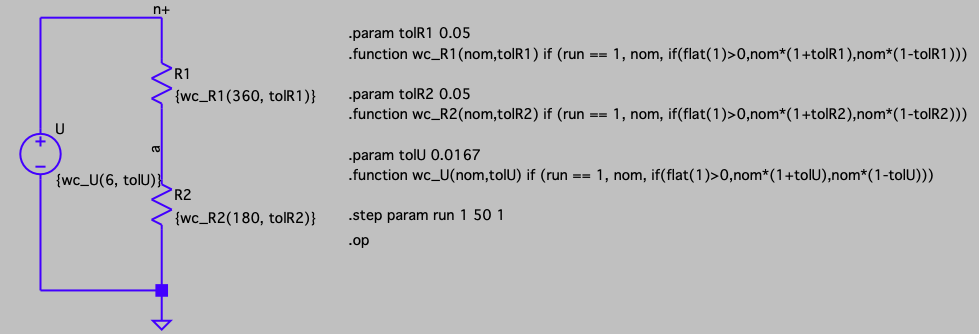
\includegraphics[width=0.6\textwidth]{laborator_01/figuri/spice_schematics_tolerante_wc}\\
		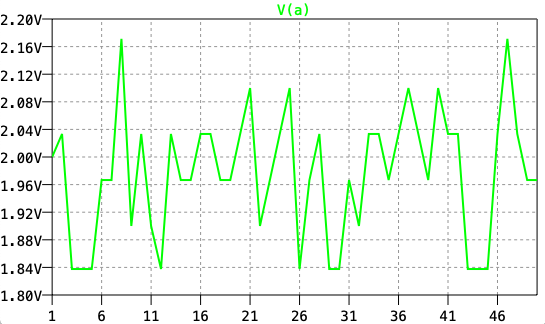
\includegraphics[width=0.6\textwidth]{laborator_01/figuri/spice_rezultate_tolerante_wc}
	\caption{Divizor de tensiune 'in gol -- m'arimi cu toleran'te, {\em worst-case scenario}, {\em schematics} 'si rezultate.}
	\label{fig:spice_tolerante_wc}
\end{figure}

\newpage

'In acest moment putem preg'ati o foaie de calcul 'in care s'a trecem valorile calculate 'si valorile rezultate 'in urma simul'arii, ca in Fig. \ref{fig:divizor_tensiune_excel2}.

\begin{figure}[h]
	\centering
	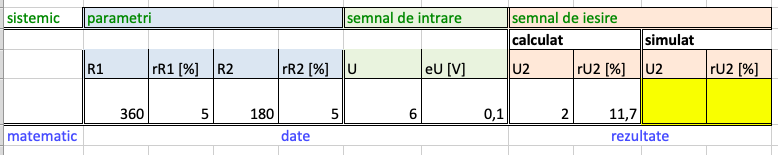
\includegraphics[width=\textwidth]{laborator_01/figuri/divizor_tensiune_excel2}
	\caption{Divizor de tensiune 'in gol -- foaie de calcul cu m'arimi calculate 'si simulate.}
	\label{fig:divizor_tensiune_excel2}
\end{figure}
\begin{exercise}%[fi'sier \textit{.cir} sau \textit{.asc}, fi'sier \textit{.xls}, 'inainte de laborator]
  Analiza'ti 'si simula'ti divizorul de tensiune 'in sarcin'a. Preg'ati'ti o foaie de calcul potrivit'a.
\end{exercise}
\begin{exercise}%[fi'sier \textit{.cir} sau \textit{.asc}, fi'sier \textit{.xls}, 'inainte de laborator]
  Analiza'ti 'si simula'ti puntea rezistiv'a. Preg'ati'ti o foaie de calcul potrivit'a.
\end{exercise}

%
% ultima actualizare: Mihai Popescu - 03/03/2020

\section{Experimente practice}

\subsection*{Aparate, componente 'si software necesar}

Pachetul ({\em kit}-ul) de laborator pe care 'il ve'ti primi con'tine: 
\begin{itemize}
\item o unitate multifunc'tional'a ANALOG DISCOVERY 2 (Fig.~\ref{fig:4_AD2_multi}, st\^anga) \cite{ad2_refman}; unitatea va fi utilizat'a ca surs'a de tensiune variabil'a 'si voltmetru;
\item un multimetru digital (Fig.~\ref{fig:4_AD2_multi}, dreapta) \cite{multimeter_manual}. Acest aparat va fi folosit pentru m'asurarea curen'tilor 'si a rezisten'telor;
\item o plac'a de test ({\em breadboard}) pe care se va executa montajul experimental, conform schemelor electrice descrise 'in lucrare;
\item un set de rezistoare din care se vor selecta doar cele necesare rezolv'arii cerin'telor lucr'arii.
\end{itemize}
'In plus, ave'ti nevoie de
\begin{itemize}
\item interfa'ta software "WaveForms" ce reprezint'a setul de instrumente virtuale asociat unit'a'tii ANALOG DISCOVERY 2 \cite{wavef_refman} ; 
\item software de simulare a circuitelor electrice - LTspice \cite{ltspice};
\item o foaie de calcul electronic'a (MsExcel, OpenOffice Calc, etc.).
\end{itemize}
\begin{figure}
	\centering
		
\includegraphics[width=0.4\textwidth]{laborator_01/figuri/4_AD2.jpg}
		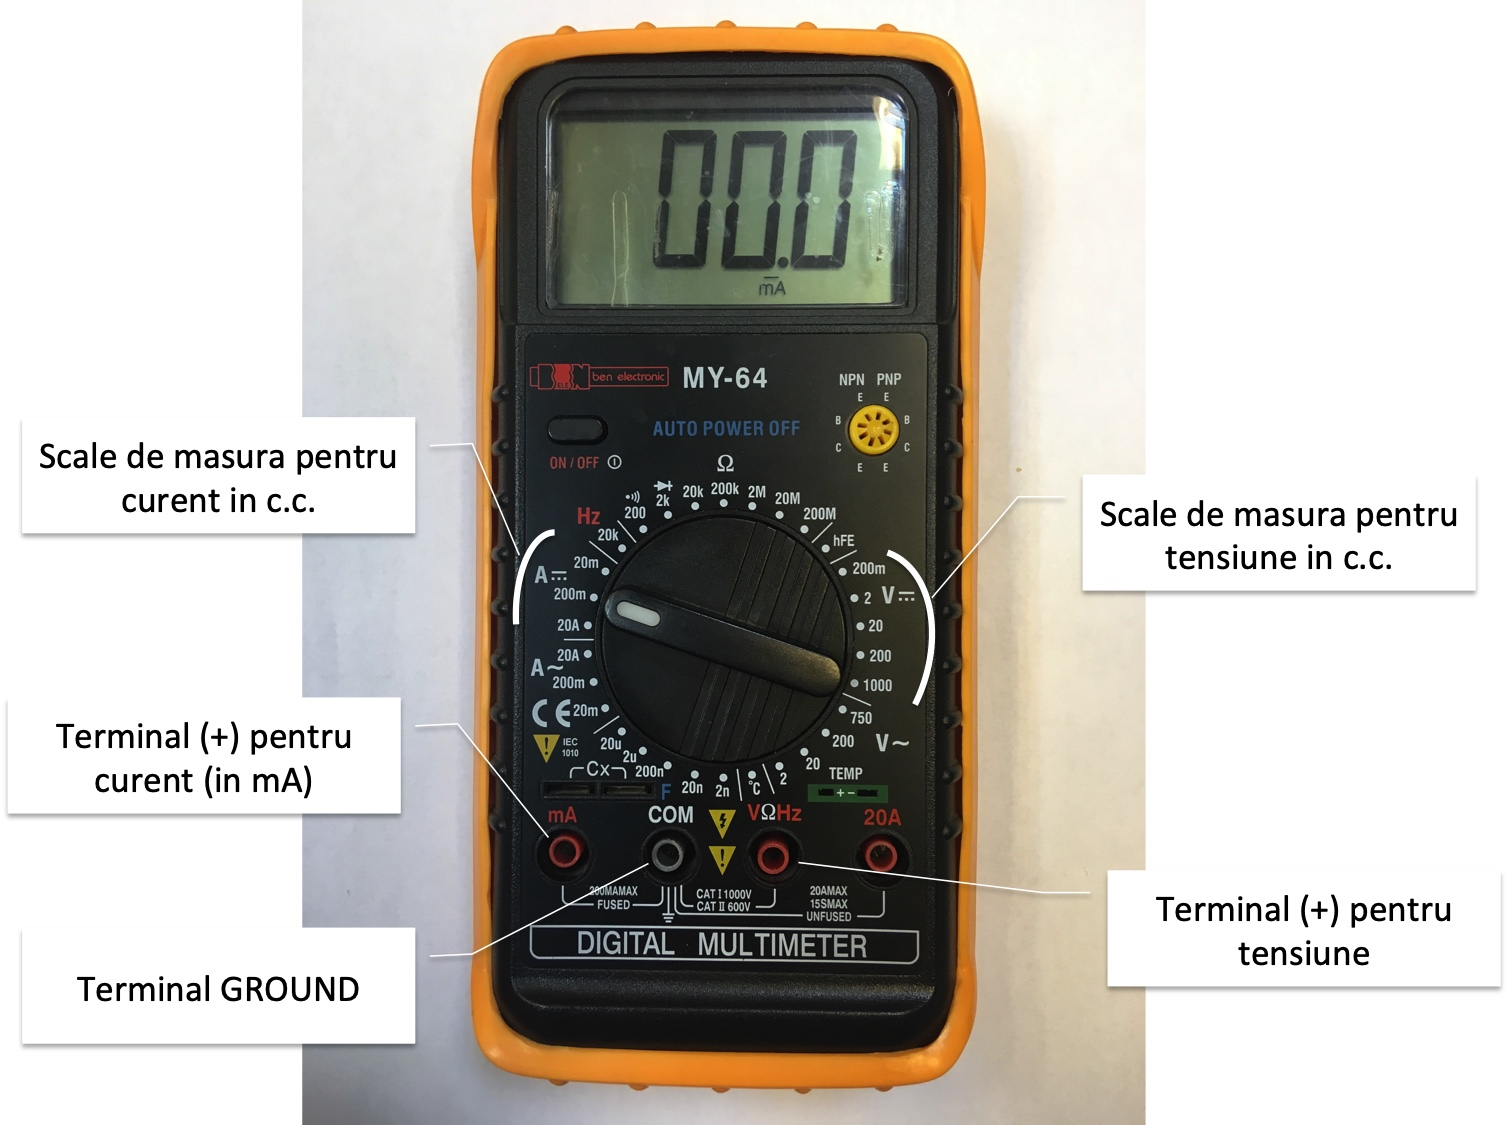
\includegraphics[width=0.5\textwidth]{laborator_01/figuri/4_multimetru_prel}
	\caption{Unitatea multifunc'tional'a ANALOG DISCOVERY 2 (st\^anga) 'si multimetrul (dreapta).}
	\label{fig:4_AD2_multi}
\end{figure}
%
%
\subsection*{Lucrarea de laborator -- pas cu pas}

Experimentele pe care trebuie s'a le realiza'ti sunt descrise mai jos. 'In paralel cu ele trebuie s'a completa'ti chestionarul corespunz'ator de pe platforma Moodle.

 \textbf{\color{red} Aten'tie!} Acest chestionar 'il pute'ti completa o singur'a dat'a, 'in timpul laboratorului. 

Deschide'ti chestionarul de pe moodle 'si 'incepe'ti a-l completa strict 'in ordinea apari'tiei problemelor de abordat. Este important'a p'astrarea acestei ordini 'intruc\^at rezultatele ob'tinute la un moment dat vor folosi pentru etape urm'atoare ale aceluia'si chestionar. 

\textbf{\color{red} Acest chestionar este un "formular de lucru" care trebui  completat pas cu pas.}

\begin{exercise}[Pasul 1. Deschiderea chestionarului 'si rezolvarea chestiunilor teoretice.]
	Deschide'ti chestionarul de pe moodle 'si  r'aspunde'ti la primele 'intreb'ari care se refer'a la teoria lucr'arii.
\end{exercise}

Fiecare student deschide un astfel de chestionar. 'Intreb'arile teoretice primite sunt, 'in general, diferite. Pute'ti lucra 'in echip'a pentru a decide r'aspunsurile corecte.

%
% -------------- Q1 ----------------
%
\begin{exercise}[Pasul 2. Preg'atirea componentelor.]
	'Inaintea 'inceperii p'ar'tii practice a oric'arei lucr'ari de laborator este necesar'a inventarierea componentelor cu care se va realiza montajul experimental. 'In acest scop va trebui s'a determina'ti, pe baza codului culorilor (Fig.~\ref{fig:rezistente_cod_culori}), valorile rezisten'telor 'inscrise pe corpurile rezistoarelor din kit-ul primit. Pentru validarea corectitudinii citirilor pute'ti folosi func'tia de ohmetru a multimetrului digital. Constata'ti faptul c'a valorile m'asurate difer'a de cele 'inscrise prin codul culorilor, 'in limita toleran'tei de fabrica'tie  indicat'a tot printr-o culoare.  
\end{exercise}
%\todoINFO{Aici ar trebui o referin't'a c'atre ecua'tiile care dau marginile erorii absolute care NU sunt etichetate inc'a}
\begin{observ}
	Pe foaia de calcul electronic'a pute'ti verifica, pentru fiecare rezistor, 'inscrierea valorii determinate cu ohmetrul 'in limitele toleran'tei specificate pe corpul rezistorului prin cod de culoare; verificarea se poate face prin implementarea, pe foaia de calcul electronic'a, a rela'tiilor din capitolul dedicat propag'arii erorilor. 
\end{observ}
%
\begin{figure}
	\centering
		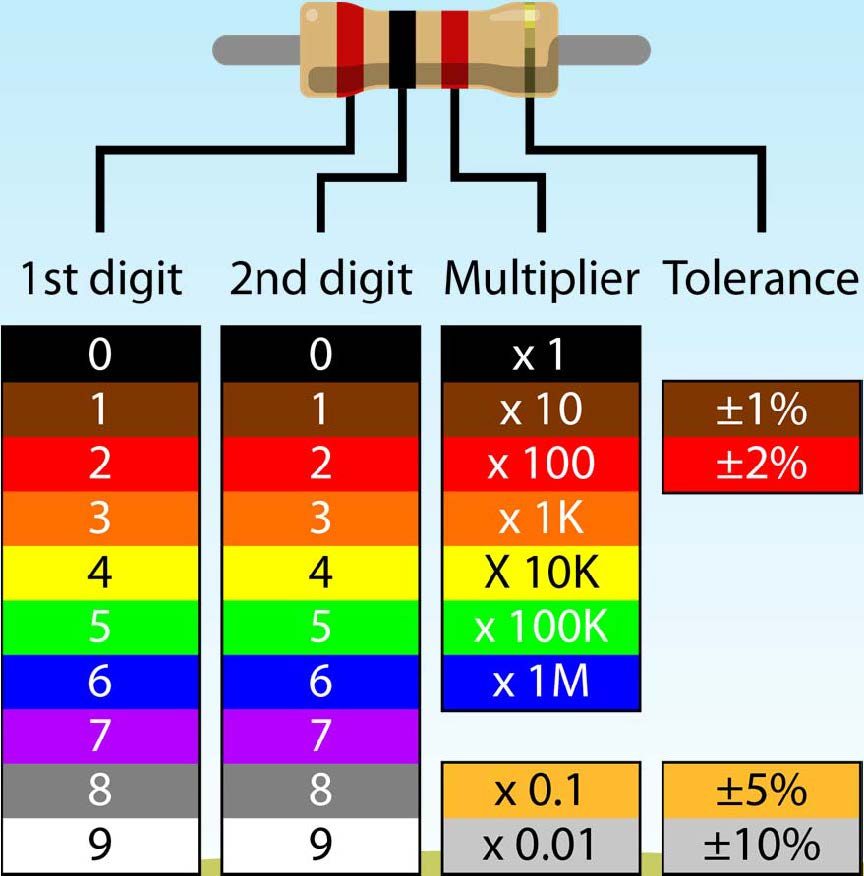
\includegraphics[width=0.4\textwidth]{laborator_01/figuri/rezistente_cod_culori}
	\caption{Codul de culori pentru un rezistor are 4 benzi. Primele dou'a benzi indic'a primele dou'a cifre semnificative, iar a treia band'a reprezinta puterea lui 10 cu care se multiplic'a num'arul 'intreg de 2 cifre codificat de primele dou'a benzi. A patra band'a reprezinta toleran'ta 'in procente. Valoarea rezisten'tei din figur'a este de $20 \cdot 10^2 \, \Omega = 2 \, k\Omega$, cu o toleran't'a de 5\%. Pe scurt: $2 \, k\Omega \pm 5\%$.}
	\label{fig:rezistente_cod_culori}
\end{figure}
%
% ------------------ Q2 -----------------
%
\begin{exercise}[Condi'tii de proiectare a circuitului] \label{Q2}
Din setul de rezistoare primite selecta'ti-le pe cele care v'a permit realizarea unui divizor cu  un raport $k = U_1/U_2$ indicat 'in enun'tul exerci'tiului. Alegerea trebuie s'a fie f'acut'a astfel 'inc\^at curentul prin divizor s'a nu fie mai mic de o valoare  $I_{\mathrm{div}_{\mathrm{min}}}$   indicat'a 'in formular. 
\end{exercise}
%
\begin{indicatie}
Determina'ti mai 'int\^ai rezisten'ta total'a maxim'a a divizorului din rela'tia 
\begin{equation} \label{rdivmax}
	(R_1 + R_2)\leq U_1/I_{\mathrm{div}_{\mathrm{min}}}.
\end{equation}
 'In continuare, utiliz\^and rela'tiile \eqref{retine1}, determina'ti raportul dintre cele dou'a rezisten'te, imediat rezult\^and 'si valorile teoretice pentru fiecare dintre ele. 'In final nu r'am\^ane dec\^at s'a selecta'ti, din setul disponibil, rezistoarele care au cele mai mari rezisten'te apropiate de valorile teoretice determinate, dar mai mici dec\^at acestea, a.'i. s'a fie satisf'acut'a condi'tia \eqref{rdivmax}. 
\end{indicatie}
%
% ---------------- Q3 -----------------
%
\begin{exercise}[Verificarea teoretic'a a circuitului proiectat] \label{Q3}
Aplic\^and rela'tia \eqref{eq:tensiune_intrare_gol}, determina'ti valorile curentului prin divizorul de tensiune $I_{\mathrm{div}}$, respectiv a tensiunii $U_2$ de la ie'sirea acestuia, 'in condi'tiile 'in care tensiunea de intrare este cea specificat'a la exerci'tiul \ref{Q2}. Pentru $R_1$, respectiv $R_2$ folosi'ti valorile rezisten'telor alese 'in acela'si exerci'tiu.  
\end{exercise}
%
% ---------------- Q4 -----------------
%
\begin{exercise} [Simularea unui model virtual al circuitului proiectat] \label{Q4}
Folosind una din tehnicile descrise 'in sec'tiunea  \ref{sec:ltspice}, conform 
Fig.~ \ref{fig:spice_ex1_3} 'si/sau Fig.~\ref{fig:spice_ex1_4}, simula'ti func'tionarea 'in gol a divizorului de tensiune, cu valorile date, respectiv determinate la exerci'tiul \ref{Q2}. Completa'ti formularul de lucru cu rezultatele ob'tinute din simulare.
\end{exercise}
%
% ---------------- Q5 -----------------
%
\begin{exercise} [Realizarea circuitului pe placa de test 'si verificarea parametrilor func'tionali la mersul 'in gol] \label{Q5}
Pentru a efectua cu u'surin't'a procedurile de m'asurare ce vor urma, precum 'si pentru a reduce posibilit'a'tile de a gre'si, este foarte important s'a desena'ti pe h\^artie schema divizorului, etichet\^and fiecare nod de circuit cu num'arul nodului corespunz'ator de pe placa de test. 'In acest mod ve'ti putea:
\begin{itemize}
\item detecta cu u'surin't'a eventuale erori de montaj;
\item stabili clar noduri importante utile pentru a m'asur'a curen'ti, tensiuni, poten'tiale;
\item urm'ari 'in mod coerent 'si ordonat toate modific'arile pe care le ve'ti opera 'in topologia circuitului experimental.  
\end{itemize}
%
O recomandare a unei posibile a'sez'ari (poz'ari) a componentelor este dat'a 'in Fig.~\ref{fig:4_divizor1_bb}. Tensiunea de intrare $U_1$ este asigurat'a din sursa de tensiune continu'a pozitiv'a a unit'a'tii AD2, 'intre bornele $V+$ 'si $\mathrm{GND}$. Pentru determinarea curentului prin divizorul de tensiune, conecta'ti multimetrul (setat pe func'tia 200mA/cc) 'in serie cu gruparea $R_1 - R_2$. Pentru m'asurarea tensiunii $U_2$, folosi'ti primul canal de m'asur'a al AD2 'intre bornele $+1$ 'si $-1$.
\begin{retine}
	{\color{blue}
Orice modificare 'in schem'a se va efectua fie cu portul USB al AD2 deconectat, fie cu sursele de tensiune oprite 
("MASTER ENABLE" - 'in stare $\mathrm{OFF}$).
}
\end{retine}
Pentru efectuarea montajului 'si a m'asur'arilor urma'ti urm'atorii pa'si:
\begin{enumerate}
\item Asigura'ti-v'a c'a AD2 are cablul USB deconectat din calculator;
\item Realiza'ti montajul experimental conform schemei;  
\item Verifica'ti corectitudinea conexiunilor (coresponden'ta dintre schem'a 'si montaj); dac'a nu sunte'ti siguri pe ce a'ti realizat practic, discuta'ti cu profesorul 'indrum'ator;
\item Conecta'ti cablul AD2 'in portul USB al calculatorului;
\item Lansa'ti panoul virtual de instrumente al AD2 din meniul \textit{Windows $->$ Digilent $->$ WaveForms};
\item Dup'a ce interfa'ta porne'ste, se va conecta automat la AD2; acest lucru este confirmat de o diod'a luminiscent'a (LED) care se aprinde intermitent 'in unitatea AD2;
\item Deschide'ti interfa'ta voltmetrului - $Voltage$ 'si activa'ti-o cu "click" pe butonul $Run$;
\item Deschide'ti interfa'ta surselor de tensiune ("Supplies") 'si 'in fereastra \textit{Voltage} a primei surse, seta'ti tensiunea $U_1$ la valoarea indicat'a la exerci'tiul \ref{Q2};
\item Activa'ti sursa de tensiune prin "click" pe \textit{"Positive Supply (V+) Rdy"}, iar apoi pe \textit{"Master Enable"} care din starea OFF va trece 'in starea ON.
\item Dac'a totul este corect, pe afi'sajul DC al voltmetrului 1 va ap'area tensiunea $U_2$, iar pe afi'sajul multimetrului va ap'area intensitatea curentului prin divizor.
\item Cele dou'a valori trebuie s'a fie apropiate de valorile determinate din ecua'tii 'si prin simulare cu LTspice; dac'a acest lucru nu se 'int\^ampl'a, verifica'ti din nou corectitudinea montajului, respectiv valorile componentelor utilizate;
\item Verifica'ti dac'a intensitatea curentului prin divizor este mai mare sau egal'a cu $I_{\mathrm{div}_{\mathrm{min}}}$;
\item {\color{blue}{Pentru determinarea cu precizie bun'a a tensiunii de ie'sire $U_2$, elimina'ti ampermetrul din circuit, 'intruc\^at rezisten'ta sa intern'a modific'a raportul de divizare a divizorului de tensiune}};
\item Nota'ti pe formularul de lucru valorile m'asurate;
\item Dezactiva'ti sursa de alimentare (\textit{"Master Enable"} 'in stare OFF). 
\end{enumerate}
\end{exercise}
%

\begin{observ}
		\begin{itemize}
			\item 	{\color{blue}
				Orice modificare 'in schem'a se va efectua fie cu portul USB al AD2 deconectat, fie cu sursele de tensiune oprite 
				("MASTER ENABLE" - 'in stare $\mathrm{OFF}$).}
\item nota'ti-v'a pe foaia de calcul electronic'a rezultatele m'asur'arilor;
\item ca schem'a de referin't'a, 'in loc de schema pe h\^artie, pute'ti folosi 'si schema generat'a cu interfa'ta grafic'a a LTspice, cu condi'tia de a eticheta 'si acolo nodurile (butonul \textit{Label Net}) cu acelea'si etichete numerice ca ale nodurilor corespunz'atoare de pe placa de test.
\end{itemize} 
\end{observ}
%
\begin{figure}
	\centering
		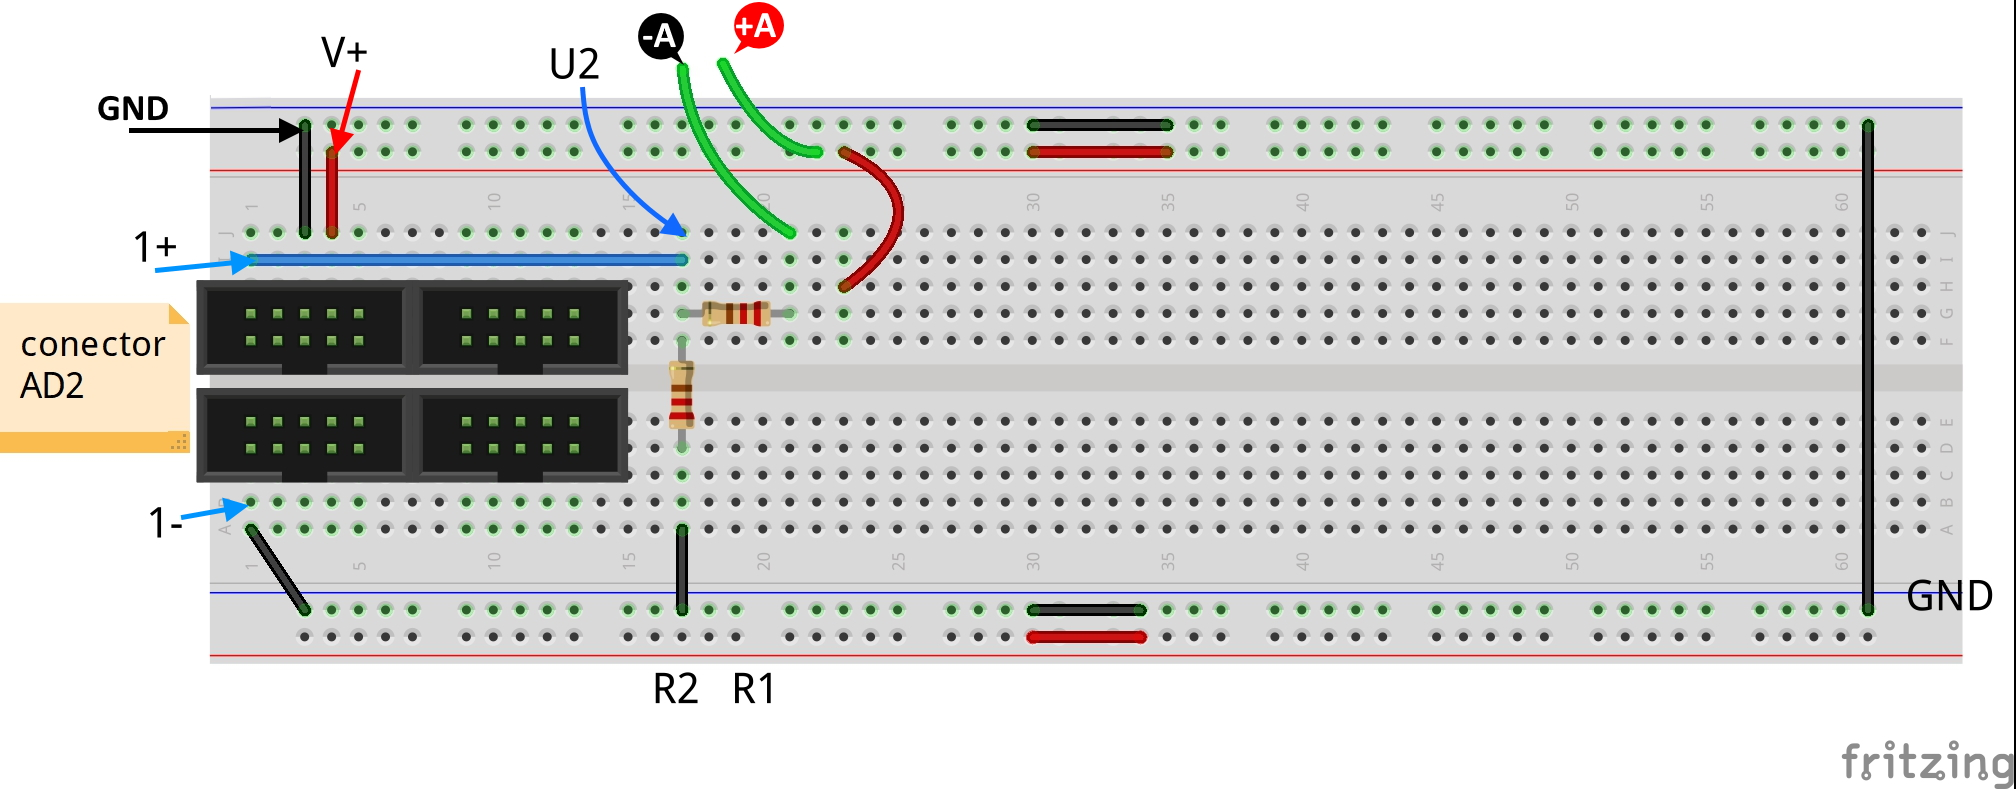
\includegraphics[width=0.8\textwidth]{laborator_01/figuri/4_divizor_1_bb}
	\caption{Amplasamentul componentelor pentru divizorul de tensiune. Curentul se m'asoar'a conect\^and multimetrul pe scara de mA/cc 'intre bara de alimentare V+ (ro'sie) 'si R1. Tensiunea se m'asoar'a prin canalul de m'asur'a 1 al AD2, conect\^and intrarea 1- la bara GND (albastr'a), 'si intrarea 1+ la ie'sirea divizorului de tensiune.}
	\label{fig:4_divizor1_bb}
\end{figure}
%
% ---------------- Q6 -----------------
%
\begin{exercise}[Stabilirea modului de testare a circuitului 'in sarcin'a] \label{Q6}
	Determina'ti rezisten'ta de sarcin'a $R_s$, astfel 'inc\^at $I_s \leq 50 \cdot I_{\mathrm{div}}$. Unde pentru $I_{div}$ considera'ti valoarea m'asurat'a la exerci'tiul \eqref{Q5}. \c{T}ine'ti cont c'a rezisten'ta are o toleran't'a de $\pm 5\%$.	
\end{exercise}
%
\begin{indicatie}
	Pentru determin'arile de mai jos, folosi'ti foaia electronic'a de calcul.
	Calcula'ti mai 'int\^ai limita inferioar'a teoretic'a a rezisten'tei de sarcin'a din condi'tia:
\begin{equation} \label{conditie_Rs}
	 R_s \geq 50 \cdot I_{\mathrm{div}_{\mathrm{masurat}}}.
\end{equation}
Determina'ti apoi valoarea teoretic'a ce ar putea fi 'inscris'a pe un rezistor cu toleran't'a $\pm 5\%$ astfel ca, 'in cel mai defavorabil caz, condi'tia \eqref{conditie_Rs} s'a fie respectat'a.
\end{indicatie}
%
% ---------------- Q7 -----------------
%
\begin{exercise}[Testarea circuitului 'in sarcin'a] \label{Q7} %, conform modului de testare stabilit] \label{Q7}
	Alege'ti rezistorul, cu cea mai mic'a valoare de rezisten't'a, disponibil 'in kit-ul primit, care 'indepline'ste condi'tia impus'a 'in exerci'tiul \eqref{Q6}. Determina'ti intensitatea curentului de sarcin'a teoretic folosind pentru rezisten't'a valoarea 'inscris'a pe rezistorul ales:
\begin{equation} \label{is_teoretic}
	I_{s_{\mathrm{teoretic}}} = U_{2_{\mathrm{masurat}}} / R_{s_{\mathrm{real}}}.
\end{equation}
	Conecta'ti rezistorul de sarcin'a ales, la ie'sirea divizorului deja construit.  M'asura'ti curentul de sarcin'a $I_{s_{\mathrm{masurat}}}$ 'si calcula'ti eroarea relativ'a fa't'a de valoarea teoretic'a determinat'a. Efectua'ti aceea'si compara'tie 'si pentru tensiunea de ie'sire $U_2$. Selecta'ti ('in formularul de lucru) gama de valori corespunz'atoare erorilor relative ob'tinute pentru cele dou'a m'arimi.	
\end{exercise}
%
\begin{observ}
$I_s$ se m'asoar'a cu multimetrul setat pe scala de m'asur'a 2 mA/cc, respectiv tensiunea cu ajutorul canalului de m'asur'a 1 al AD2;
\begin{itemize}
	\item 	{\color{blue}
		Orice modificare 'in schem'a se va efectua fie cu portul USB al AD2 deconectat, fie cu sursele de tensiune oprite 
		("MASTER ENABLE" - 'in stare $\mathrm{OFF}$).}
\item {\color{blue} Este deosebit de important s'a respecta'ti procedurile de lucru indicate la exerci'tiul \ref{Q5}; }  
\item Nota'ti-v'a pe foaia de calcul electronic'a rezultatele m'asur'arilor;
\end{itemize}
\end{observ}
%
\begin{indicatie}
'In Fig.~\ref{fig:4_divizor_sarcina} este recomandat'a o posibil'a dispunere a componentelor pentru m'asur'arile propuse. {\color{blue} De ce, 'in acest caz, nu este neap'arat necesar'a eliminarea ampermetrului atunci c\^and se m'asoar'a tensiunea de ie'sire $U_2$?}
\end{indicatie}
%
\begin{figure}
	\centering
		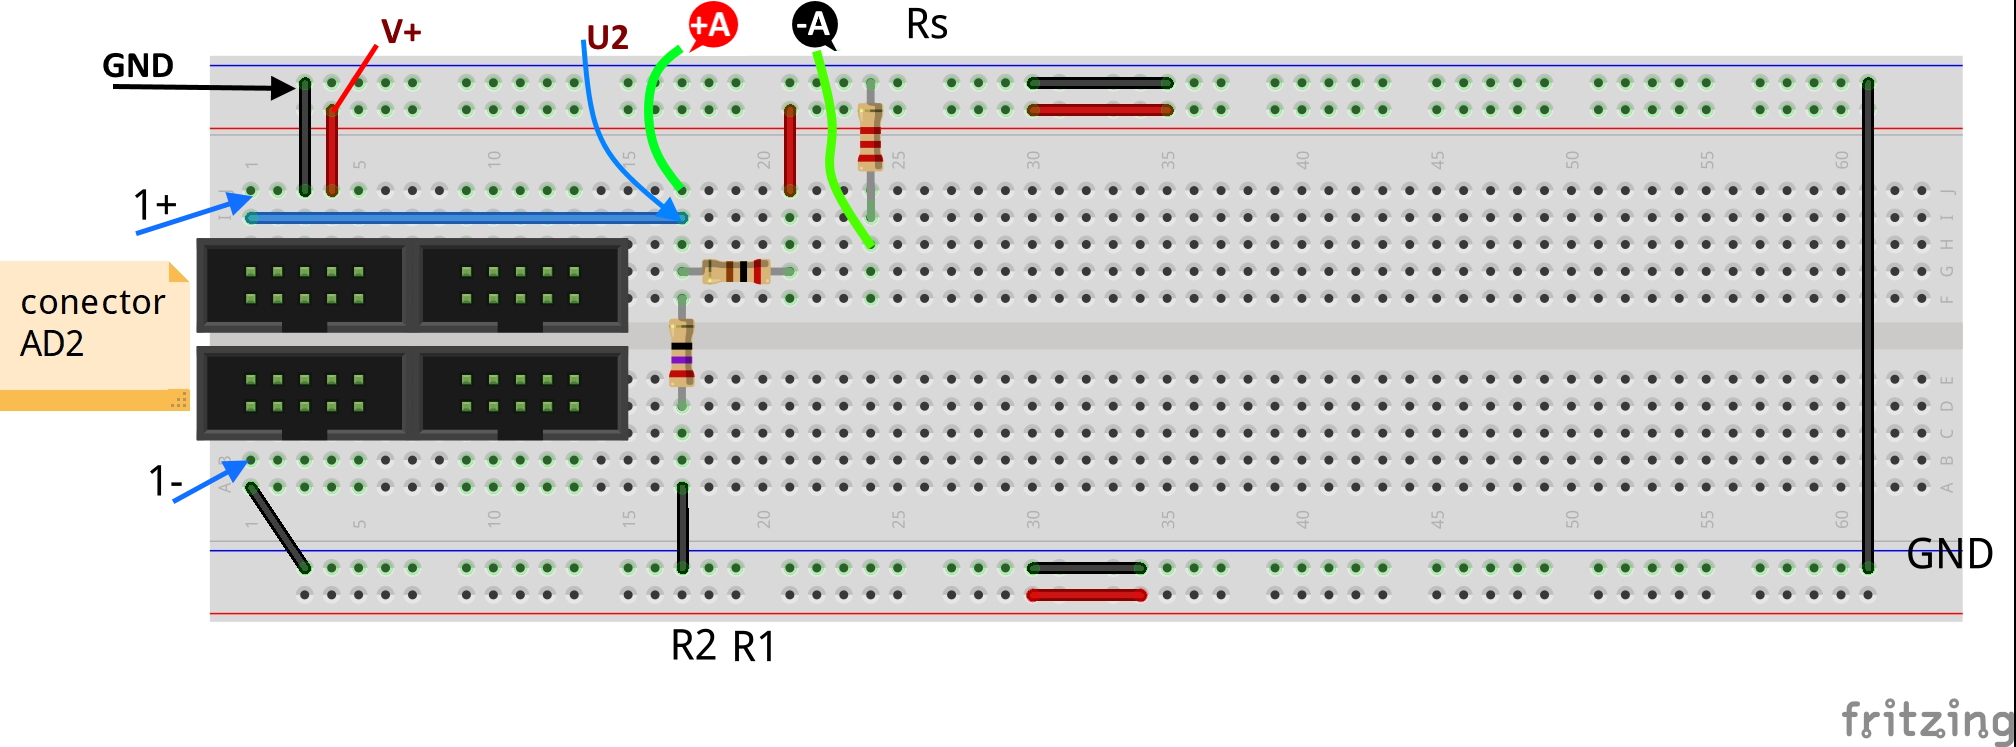
\includegraphics[width=0.8\textwidth]{laborator_01/figuri/4_divizor_sarcina_bb}
	\caption{Montaj pentru m'asurarea parametrilor electrici de ie'sire ai divizorului de tensiune 'in sarcin'a.}
	\label{fig:4_divizor_sarcina}
\end{figure}
%
% ---------------- Q8 -----------------
%
\begin{exercise} [Simularea unui model virtual al circuitului la func'tionarea 'in sarcin'a] \label{Q8}
Folosind una din tehnicile descrise 'in sec'tiunea  "LTspice", conform Fig.~\ref{fig:spice_ex1_3} 'si/sau Fig.~\ref{fig:spice_ex1_4}, simula'ti func'tionarea 'in sarcin'a a divizorului de tensiune, cu valorile alese pentru rezisten'te, respectiv determinate la exerci'tiile \ref{Q2} 'si \ref{Q7}. Completa'ti formularul de lucru cu rezultatele ob'tinute din simulare.
\end{exercise}
%
% ---------------- Q9 -----------------
%
\begin{exercise} [Aplica'tii ale divizorului de tensiune: puntea rezistiv'a] \label{Q9}
Alege'ti din kit-ul de laborator alte dou'a rezistoare, cu rezisten'tele $R_4 > R_3$, cu care s'a pute'ti construi un al doilea divizor de tensiune. Acesta va fi montat 'in paralel cu primul astfel 'inc\^at s'a formeze o punte echilibrat'a (vede'ti 'si schema electric'a de pe formularul de lucru).  
Alimenta'ti puntea cu tensiunea $U_1$ indicat'a la exerci'tiul \ref{Q2} 'si m'asura'ti curentul total $I_p$ prin puntea rezistiv'a astfel construit'a. Selecta'ti intervalul potrivit din formularul de lucru. 
\end{exercise}

\begin{observ}
$I_p$ se m'asoar'a cu multimetrul setat pe scala de m'asur'a 200 mA/cc;
\begin{itemize}
	\item 
		{\color{blue}
		Orice modificare 'in schem'a se va efectua fie cu portul USB al AD2 deconectat, fie cu sursele de tensiune oprite 
		("MASTER ENABLE" - 'in stare $\mathrm{OFF}$).}
\item {\color{blue} Este foarte important s'a respecta'ti procedurile de lucru indicate la exerci'tiul \ref{Q5}; }  
%\item \textbf{ORICE MODIFICARE IN SCHEMĂ SE VA EFECTUA FIE CU PORTUL USB AL AD2 DECONECTAT, FIE CU SURSELE DE TENSIUNE OPRITE ("MASTER ENABLE" - 'in stare $OFF$)}.
\item Nota'ti-v'a pe foaia de calcul electronic'a rezultatele m'asur'arilor;
\end{itemize}
\end{observ}
%
\begin{indicatie}
Pentru ca puntea s'a fie echilibrat'a este suficient ca cele dou'a divizoare conectate 'in paralel s'a aib'a acela'si raport de divizare.
'In Fig.~\ref{fig:4_punte_rez} este recomandat'a o posibil'a dispunere a componentelor.
\end{indicatie}
%
\begin{figure}
	\centering
		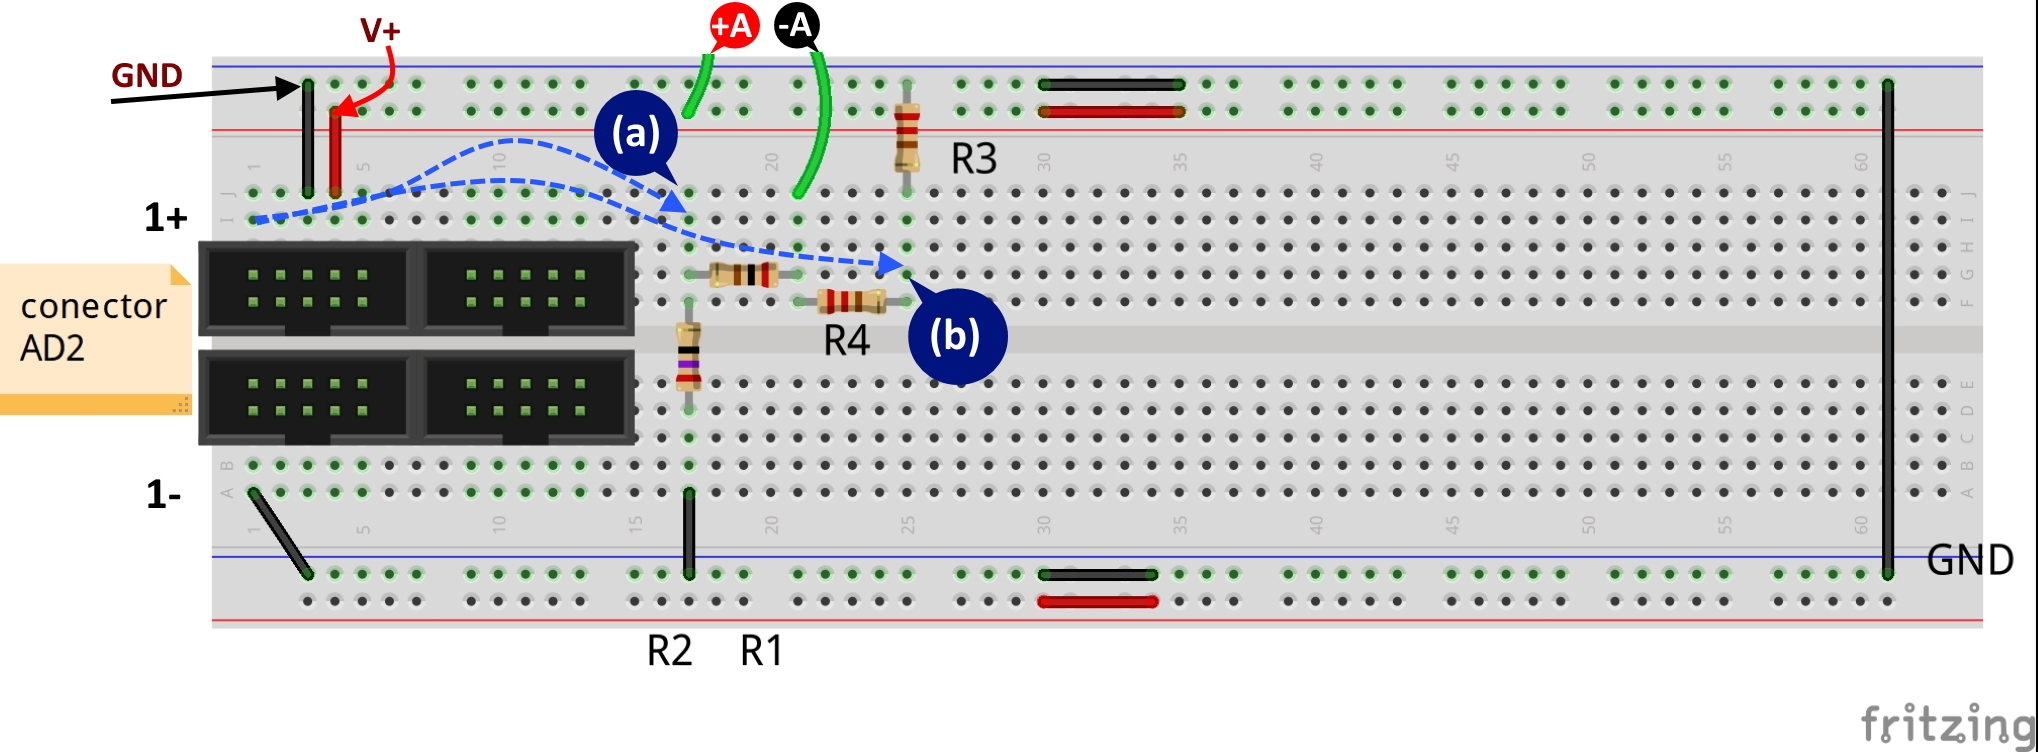
\includegraphics[width=0.8\textwidth]{laborator_01/figuri/4_punte_rez_bb}
	\caption{Montaj pentru m'asurarea parametrilor electrici de ie'sire ai pun'tii rezistive  'in sarcin'a.}
	\label{fig:4_punte_rez}
\end{figure}
%
% ---------------- Q10 -----------------
%
\begin{exercise} [Simularea modelului virtual al aplica'tiei] \label{Q10}
Folosind una din tehnicile descrise 'in sec'tiunea  \ref{sec:ltspice}, conform Fig.~\ref{fig:spice_ex1_3} 'si \ref{fig:spice_ex1_4}, simula'ti func'tionarea 'in sarcin'a a pun'tii rezistive construite. Completa'ti formularul de lucru cu rezultatele ob'tinute din simulare.
\end{exercise}
%
% ---------------- Q11 -----------------
%
\begin{exercise} [Caracteristici principale ale func'tion'arii aplica'tiei] \label{Q11}
Pentru acela'si montaj experimental de la exerci'tiul \ref{Q9} m'asura'ti tensiunea 'intre nodurile $(a)$ 'si $(b)$ ale pun'tii rezistive (Fig.~\ref{fig:4_punte_rez}). R'aspunde'ti cerin'telor specificate 'in formularul de lucru pentru acest exerci'tiu. 
\end{exercise}
%
% ---------------- Q12 -----------------
%
\begin{exercise} [Utiliz'ari ale aplica'tiei: m'asurarea de rezisten'te] \label{Q12}
Cea mai r'asp\^andit'a aplica'tie a pun'tii rezistive este cea de determinare de precizie a unor rezisten'te necunoscute; valorile necunoscute pot reprezenta rezisten'te ale unor rezistoare electrice liniare, sau rezisten'te ale unor senzori rezistivi a c'aror valoare este propor'tional'a cu m'arimi neelectrice (presiune, for't'a, temperatur'a, intensitate luminoas'a) m'asurate cu ajutorul acestor senzori. Exerci'tiul presupune m'asurarea rezisten'tei cunoscute a unui rezistor 'si compararea valorilor m'asurat'a 'si real'a. Urm'ari'ti pa'sii indica'ti 'in formularul de lucru pentru acest exerci'tiu. 
\end{exercise}
%
\begin{observ}
Rezisten'ta se m'asoar'a cu multimetrul setat pe scala de m'asur'a 2k;
\begin{itemize}
\item tensiunea $U_{ab}$ se determin'a cu ajutorul canalului de m'asur'a 1 al AD2, conect\^and nodurile (a) 'si (b) la bornele +1, respectiv -1 ale acestuia (v. fig. \ref{fig:4_punte_rez_x});
\item {\color{blue} Respecta'ti procedurile de lucru indicate la exerci'tiul \ref{Q5}; } 
\item  
	{\color{blue}
	Orice modificare 'in schem'a se va efectua fie cu portul USB al AD2 deconectat, fie cu sursele de tensiune oprite 
	("MASTER ENABLE" - 'in stare $\mathrm{OFF}$).}
\item Nota'ti-v'a pe foaia de calcul electronic'a rezultatele m'asur'arilor;
\end{itemize}
\end{observ}
%
\begin{indicatie}
'In Fig.~\ref{fig:4_punte_rez_x} este recomandat'a o posibil'a dispunere a componentelor.

Poten'tiometrul este o component'a rezistiv'a cu rezisten'ta variabil'a prin deplasarea rotativ'a sau liniar'a a unui contact mobil numit {\em cursor} 'intre dou'a contacte cu pozi'tie extrem'a: \textit{valoare 0}, respectiv \textit{valoare maxim'a}. Valoarea maxim'a este cea care caracterizeaza poten'tiometrul respectiv. Dac'a reglajul  nu este accesibil dec\^at limitat, direct pe placa de montaj, spunem c'a acest poten'tiometru este {\em semireglabil}. 
'In cazul 'in care cursorul formeaz'a un nod cu una din bornele extreme spunem c'a avem o {\em rezisten't'a variabil'a simpl'a}. 'In cazul 'in care cursorul este nelegat de contactele extreme, poten'tiometrul poate fi privit ca un divizor de tensiune, cu tensiunea de ie'sire reglabil'a 'intre 0 'si tensiunea aplicat'a 'intre bornele extreme, 'in func'tie de pozi'tia cursorului relativ la acestea din urm'a  (Fig. \ref{fig:potentiometru}).
\end{indicatie}

\newpage

\begin{figure}
	\centering
		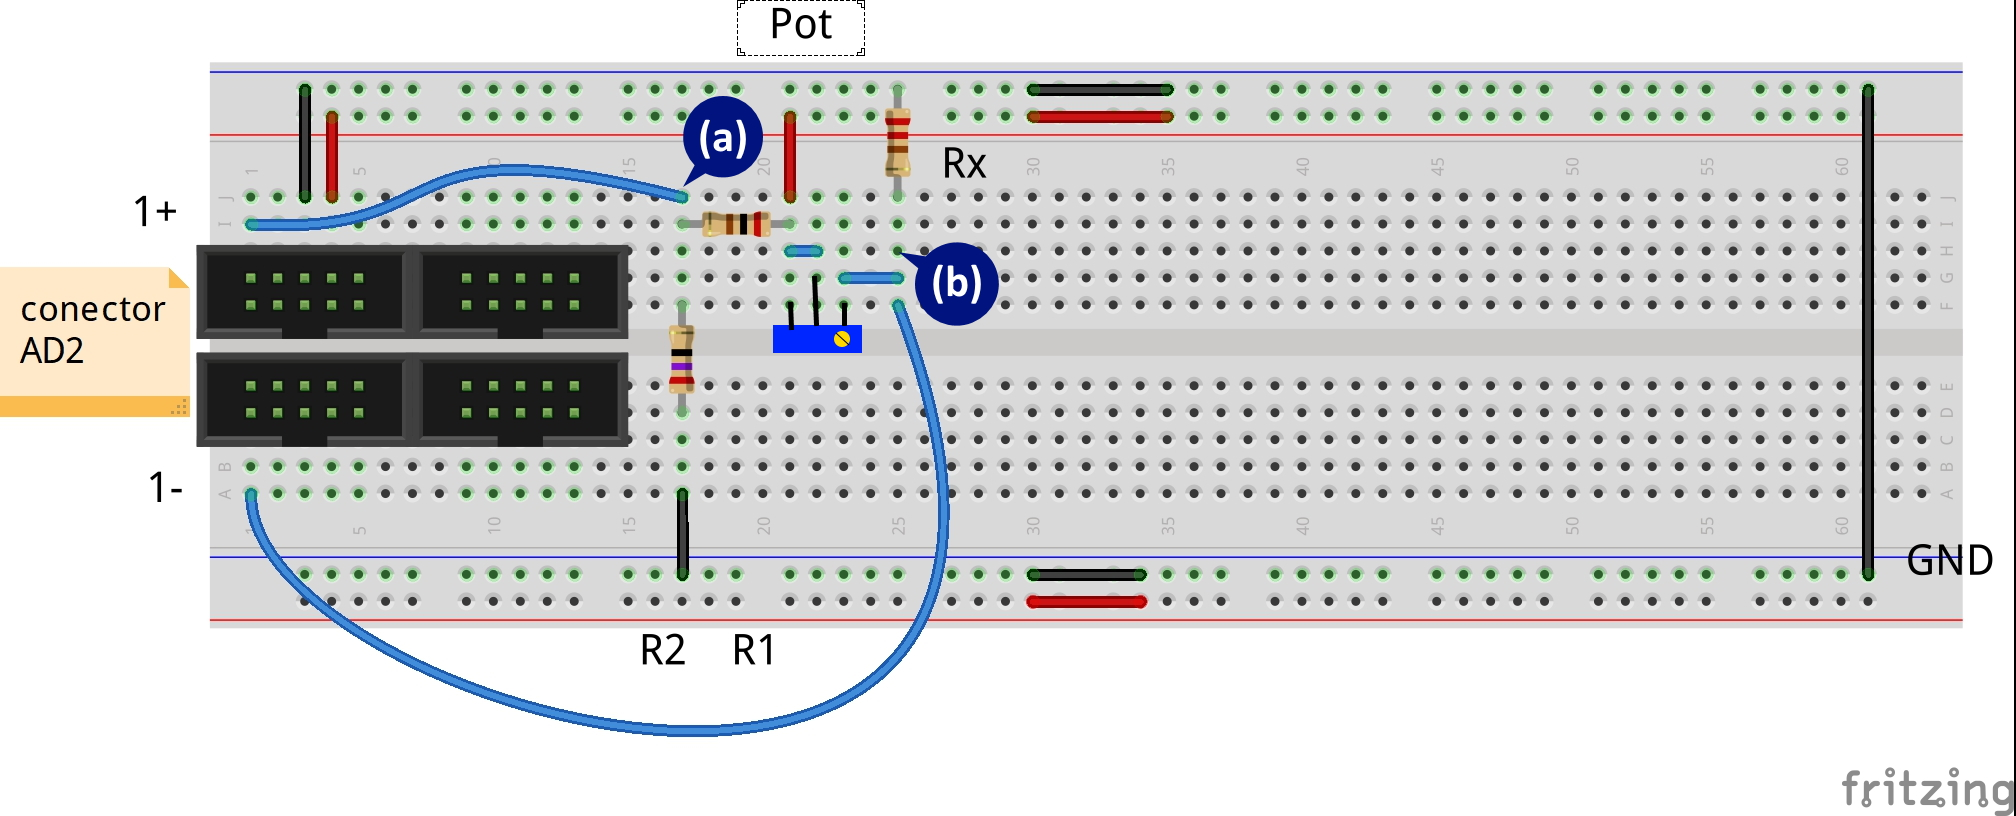
\includegraphics[width=0.8\textwidth]{laborator_01/figuri/4_punte_rez_x_bb}
	\caption{Montaj pentru m'asurarea unei rezisten'te necunoscute.}
	\label{fig:4_punte_rez_x}
%\end{figure}
%\begin{figure}
	\centering
		
\includegraphics[width=0.35\textwidth]{laborator_01/figuri/6_potentiometru0}
		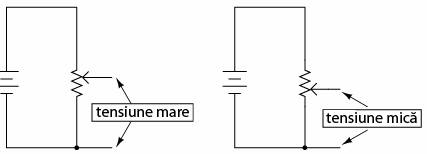
\includegraphics[width=0.45\textwidth]{laborator_01/figuri/6_potentiometru2}
	\caption{Poten'tiometrul. Tensiunea de ie'sire se modific'a 'in func'tie de pozi'tia cursorului 'intre bornele extreme. \cite{aplicatii_potentiometru}.}
	\label{fig:potentiometru}
\end{figure}
%


\begin{exercise}[Ultimul pas]
La finalul lucr'arii, revede'ti r'aspunsurile completate 'in chestionarul de laborator, finaliza'ti 'si 'inchide'ti chestionarul. Nota ob'tinut'a va fi afi'sat'a imediat.
\end{exercise}






\section{Validarea rezultatelor experimentale}

\subsection*{Influen'ta aparatelor de m'asur'a}

Orice aparat de m'asur'a introdus 'intr-un circuit schimb'a comportamentul acestuia. Acest lucru se 'int\^ampl'a din cauz'a c'a aparatele de m'asur'a nu sunt elemente ideale, ele av\^and rezisten'te interne.

'In cazul voltmetrelor, acestea fiind conectate 'intotdeauna 'in paralel cu componentele aflate sub test, orice curent prin voltmetru va modifica curentul total din circuit, duc\^and inevitabil 'si la modificarea tensiunii reale din circuit. Un voltmetru ideal are o rezisten't'a intern'a infinit'a, astfel 'inc\^at curentul care trece prin acesta s'a fie zero. 'In cazul unui voltmetru real, trebuie s'a ne 'inchipuim rezisten'ta intern'a a acestuia 'in paralel cu elementul de interes, ca o rezisten't'a de sarcin'a.
\begin{figure}[!b]
	\centering
		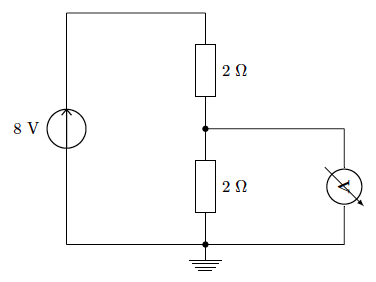
\includegraphics[width=0.55\textwidth]{laborator_01/figuri/5_divizor_cu_voltmetru}
	\caption{Divizorul de tensiune -- influen'ta aparatului de m'asur'a.}
	\label{fig:divizor_cu_voltmetru}
\end{figure}

\begin{exercise}
Ce valoare indic'a voltmetrul din Fig. \ref{fig:divizor_cu_voltmetru}, dac'a:
\begin{itemize}
\item[-] voltmetrul este ideal (rezisten't'a intern'a infinit'a)?
\item[-] voltmetrul este real (rezisten't'a intern'a va fi preluat'a din manualul multimetrului)? % \cite{multimeter_manual})?
\end{itemize}
\end{exercise}


\subsection*{Validare}

Validarea reprezint'a o etap'a extrem de important'a 'in modelare, ea confirm\^and faptul c'a simul'arile 'si experimentele au fost realizate corect. 'In aceast'a etap'a se compar'a rezultatele experimentale cu valorile analitice/simulate. 

\begin{retine}Validarea rezultatelor experimentale
Valoarea analitic'a/simulat'a $\pm$ eroarea ei trebuie s'a se afle 'in intervalul [valoare m'asurat'a -- toleran't'a, valoare m'asurat'a + toleran't'a].
\end{retine}

Pentru ca aceast'a compara'tie s'a fie relevant'a, valorile trebuie s'a aib'a acela'si num'ar de cifre semnificative. Num'arul de cifre semnificative este num'arul de cifre care sunt cunoscute cu certitudine pentru o anumit'a valoare. 

\begin{retine}
Num'arul de cifre semnificative nu este doar num'arul de cifre de dup'a virgul'a (zecimale exacte), ci num'arul total de cifre relevante! \\ 
Valoarea $2.34$ are trei cifre semnficative, 'si dou'a zecimale exacte.
\end{retine}

Num'arul $zero$ trebuie tratat special 'in raportarea cifrelor semnificative. Zerourile de dinaintea primei cifre diferite de zero nu sunt semnificative, f'ar'a s'a conteze unde este virgula (ele indic'a doar ordinul cifrelor urm'atoare 'si pot fi 'intotdeauna eliminate folosind un factor adecvat $10^k$, adic'a mut\^and virgula la dreapta). Zerourile de dup'a virgul'a sunt semnificative, 'in timp ce zerourile de dinainte de virgul'a pot fi semnificative sau nu.
 
\begin{example} Urm'atoarele valori au dou'a cifre semnificative:
$34$, $3.4$, $0.34$, $0.0034$, $3.4\cdot 10^{-4}$ 
\end{example}

\begin{example} Urm'atoarele valori au trei cifre semnificative:
$345$, $3.45$, $0.345$, $0.00345$, $3.45\cdot 10^{-4}$, $3.40$, $0.0340$, $3.40\cdot 10^{-7}$, $3.04$ , $0.000340$
\end{example}

\begin{retine}
'In raportarea unui num'ar 'intreg poate fi neclar c\^ate cifre semnificative sunt folosite. \\
Num'arul $450$ poate fi scris cu dou'a zecimale exacte: $4.5\cdot 10^2$ sau cu trei zecimale exacte: $4.50\cdot 10^2$, dar scrierea $450$ este ambigu'a din acest punct de vedere.
\end{retine}

%\textcolor{red}{$3.4\cdot 10^2$ are doua cifre semnificative ?!}

Modul de raportare a rezultatelor experimentale se face urm\^and anumite reguli.
% (mai multe detalii 'in \cite{cifre_semnificative}):

\begin{enumerate}
\item Erorile absolute ale valorilor determinate experimental nu ar trebui raportate cu mai mult de dou'a cifre semnificative.
\item O valoare 'si marginea erorii absolute asociat'a se raporteaz'a cu exact acela'si num'ar de zecimale exacte (num'ar de cifre dup'a virgul'a).
\begin{example}
Scrierea $2.4\mathrm{~V}\pm 0.16\mathrm{~V}$ implic'a faptul c'a valoarea se afl'a 'in intervalul $2.24\mathrm{~V} - 2.56\mathrm{~V}$. Dar aparatul poate m'asura valori cu o singu'ra zecimal'a exact'a, deci modul corect de raportare este $2.4\mathrm{~V}\pm 0.2\mathrm{~V}$.
\end{example}

\item At\^at valorile m'asurate c\^at 'si erorile absolute corespunz'atoare trebuie s'a aib'a aceea'si unitate de m'asur'a.
\item Raportarea trebuie s'a fie consistent'a 'in nota'tii: dac'a o valoare masurat'a este scris'a 'stiin'tific ($2.3\cdot 10^2$) atunci 'si eroarea absolut'a va fi scris'a tot 'stiin'tific.
\item La efectuarea de opera'tii elementare, rezultatul nu va avea mai multe cifre semnificative dec\^at operandul cu cele mai pu'tine cifre semnificative. Motiva'tia st'a 'in faptul c'a rezultatul nu poate fi mai precis dec\^at valoarea de intrare cea mai pu'tin precis'a. Precizia nu poate fi 'imbun'at'a'tit'a prin efectuarea de calcule. Pentru minimizarea erorilor de rotunjire, se pot utiliza mai multe cifre semnificative 'in calculele intermediare 'si se ajusteaz'a cifrele semnificative numai pentru rezultatele finale.
\begin{example}Cifre semnificative 'in opera'tii elementare: \\
$3.5 \cdot 22.3 = 78, \text{ nu } 78.05$; \\
$6.2 / 833 = 0.0074, \text{ nu } 0.007442977$; \\
$42.4 - 41.62 = 0.8$, $4256 - 24.7 = 4231$, $33.8 + 15.63 = 49.4$.
\end{example}
\end{enumerate}   

\begin{exercise}
Exemple de valorile m'asurate raportate:
\begin{itemize}
\item $0.2 \pm 0.321$ \textcolor{red}{(incorect)}
\item $0 \pm 2$ \textcolor{red}{(corect)}
\item $3.14 \pm 0.02$ \textcolor{red}{(corect)}
%\item $120$ \textcolor{red}{(incorect?)}
\item $3.1421 \pm 0.3214$ \textcolor{red}{(incorect)}
\item $(2.34 \pm 0.15)\cdot 10^{-4}$ \textcolor{red}{(corect)}
\item $(2.34 \pm 0.152)\cdot 10^{-4}$ \textcolor{red}{(incorect)}
\item $0.2 \pm 0.3$ \textcolor{red}{(corect)}
\end{itemize}
\end{exercise}


\section[Aplica'tii practice ale divizorului de tensiune]{Aplica'tii practice ale divizorului de tensiune (facultativ)}

Divizorul de tensiune are o mul'time de aplica'tii practice, fiind integrat 'in multe din dispozitivele cu care interac'tion'am zi de zi.
\begin{exercise}
C'auta'ti o aplica'tie 'in care apare un divizor de tensiune. Explica'ti principiul dup'a care este folosit.
\end{exercise}

\subsection*{Poten'tiometrul}

Una dintre utiliz'arile cele mai comune ale divizorului de tensiune o reprezint'a poten'tiometrul \cite{aplicatii_potentiometru}. Cel mai bun exemplu de poten'tiometru este butonul de reglare a volumului ata'sat unui sistem de muzic'a (Fig. \ref{fig:potentiometru}). 

Poten'tiometrul prezint'a un buton rotativ care este ac'tionat manual. Elementul mobil, numit 'si perie, face contact cu un material rezistiv dezizolat, 'in oricare dintre punctele selectate manual. Rotirea acestuia modific'a punctul de contact de pe banda rezistiv'a continu'a, astfel 'inc\^at se schimb'a valorile rezisten'telor 'si implicit coeficientul $\alpha$ de divizare 'si tensiunea de ie'sire (Fig. \ref{fig:potentiometru_tensiuni}).

Cu alte cuvinte, un poten'tiometru ac'tioneaz'a precum un divizor variabil de tensiune, iar coeficientul de divizare este dat de pozi'tia periei de-a lungul bandei rezistive.

\begin{figure}[!b]
	\centering
		
\includegraphics[width=0.35\textwidth]{laborator_01/figuri/6_potentiometru0}
		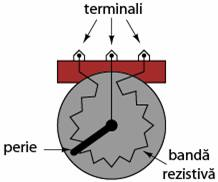
\includegraphics[width=0.3\textwidth]{laborator_01/figuri/6_potentiometru1}
	\caption{Poten'tiometrul -- mod de func'tionare} %\cite{aplicatii_potentiometru}.}
	\label{fig:potentiometru}
\end{figure}

\begin{figure}[!t]
	\centering
		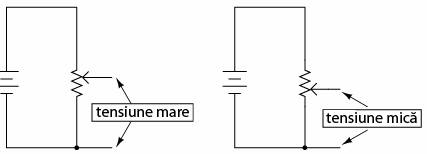
\includegraphics[width=0.65\textwidth]{laborator_01/figuri/6_potentiometru2}
	\caption{Poten'tiometrul -- tensiunea preluat'a se modific'a 'in func'tie de pozi'tia punctului de contact 'intre perie 'si banda rezistiv'a.} % \cite{aplicatii_potentiometru}.}
	\label{fig:potentiometru_tensiuni}
\end{figure}

\subsection*{Senzori rezistivi}

O mare parte din senzorii din lumea real'a sunt dispozitive rezistive \cite{aplicatii_senzori_rezistivi}. S'a lu'am exemplul unui senzor de control al luminii (fotocelul'a), care poate aprinde sau stinge becul unei veioze/lustre automat, 'in func'tie de lumina ambiental'a. Fotocelula con'tine o rezisten'ta variabil'a, propor'tional'a cu cantitatea de lumin'a captat'a.

Tensiunea fiind mult mai u'sor de m'asurat dec\^at rezisten'ta, pentru determinarea rezisten'tei fotocelulei se adaug'a un alt rezistor (cu rezisten'ta fix'a 'si cunoscut'a) 'in circuit 'in serie cu senzorul, form\^andu-se astfel un divizor de tensiune. Prin m'asurarea tensiunii de ie'sire, rezisten'ta senzorului poate fi calculat'a u'sor, folosind rela'tiile divizorului de tensiune (Fig. \ref{fig:senzor_rezistiv}).

\begin{example}
O fotocelul'a are rezisten'ta variabil'a 'intre $1~\mathrm{k\Omega}$ la lumin'a 'si aproximativ $10~\mathrm{k\Omega}$ la 'intuneric. Dac'a se monteaz'a 'in serie o rezisten't'a de valoare fixat'a la $5.6~\mathrm{k\Omega}$ 'si se m'asoar'a tensiunea de ie'sire, se poate determina valoarea rezisten'tei variabile 'si a nivelului de lumin'a asociat (tabelul \ref{tab:senzori_rezistivi}).

  \begin{center}
    \begin{tabular}{ccccc}\label{tab:senzori_rezistivi}
      Nivel lumin'a & $R_2$ (senzor) & $R_1$ (fixat) & $\alpha=\frac{R_1}{R_2}$ & $V_\mathrm{out}$ (m'asurat) \\
      \midrule
      Lumin'a & $1~\mathrm{k\Omega}$ &  $5.6~\mathrm{k\Omega}$ & $5.6$ & 0.76 V \\
      Semiobscur &  $7~\mathrm{k\Omega}$ &  $5.6~\mathrm{k\Omega}$ & $0.8$ & 2.78 V \\
      'Intuneric &  $10~\mathrm{k\Omega}$ &  $5.6~\mathrm{k\Omega}$ & $0.56$ & 3.21 V \\
    \end{tabular}
  \end{center}
\end{example}

\begin{figure}[!b]
	\centering
		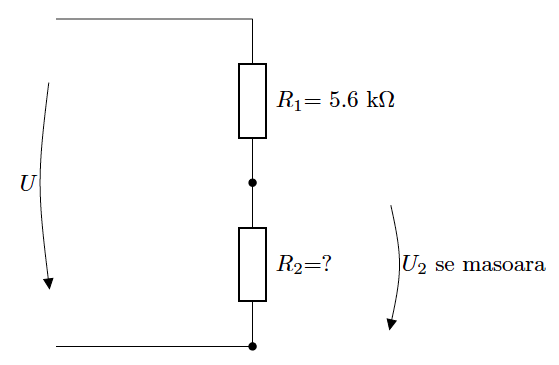
\includegraphics[width=0.45\textwidth]{laborator_01/figuri/6_senzor_rezistiv}
	\caption{Senzor rezistiv. Valoarea rezisten'tei $R_2$ a senzorului poate fi determinat'a prin crearea unui divizor de tensiune.}
	\label{fig:senzor_rezistiv}
\end{figure}

Alte exemple de acest tip sunt senzori care con'tin rezisten'te sensibile la umiditate, temperatur'a, for'te.

\subsection*{Puntea Wheatstone}

Puntea Wheatstone \cite{aplicatii_punte_wheatstone} (descris'a 'in sec'tiunea \ref{subsection:puntea_rezistiva}) a fost ini'tial dezvoltat'a de Charles Wheatstone pentru a m'asura valorile unor rezisten'te 'si ca mijloc de calibrare a instrumentelor de m'asurare (voltmetre, ampermetre).

Puntea este \textit{'in echilibru} dac'a $V_a=V_b$, ceea ce se 'int\^ampl'a dac'a rela'tia dintre rezisten'te este $R_1 R_x = R_2 R_3$. Pe acela'si principiu ca senzorii rezistivi, dac'a una dintre rezisten'te este variabil'a (de exemplu cu valoarea dependent'a de lumin'a), valoarea ei poate fi determinat'a prin echilibrarea pun'tii 'si folosirea rela'tiei 'intre rezistoare pentru o punte echilibrat'a (Fig. \ref{fig:punte_Wheatstone}).

De'si ast'azi multimetrele digitale reprezint'a cea mai simpl'a modalitate de a m'asura o rezisten't'a, puntea Wheatstone poate fi utilizat'a 'in continuare pentru a m'asura valori foarte mici ale rezisten'telor (de ordinul miliohmilor).

\begin{figure}[!t]
	\centering
		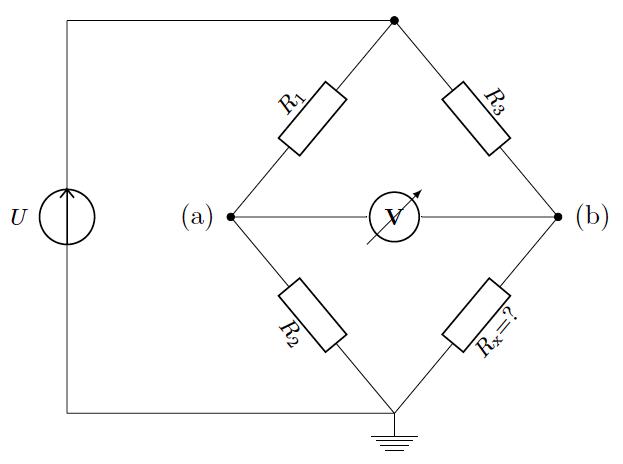
\includegraphics[width=0.45\textwidth]{laborator_01/figuri/6_punte_Wheatstone}
	\caption{Puntea Wheatstone. Valoarea rezisten'tei $R_\mathrm{x}$ se determin'a prin echilibrarea pun'tii 'si folosind rela'tia 'intre rezistoare pentru punte echilibrat'a.}
	\label{fig:punte_Wheatstone}
\end{figure}

\section[Proiectarea unui divizor de tensiune]{Proiectarea unui divizor de tensiune (facultativ)}

'In sec'tiunea \ref{subsection:ca_sisteme} (Fig. \ref{fig:divizor_tensiune_gol_sistem}) am considerat divizorul de tensiune ca un sistem, 'in care (tensiunea de) ie'sire depinde de (tensiunea de) intrare prin func'tia de transfer $H = \frac{1}{1+\alpha}$, unde $\alpha = \frac{R_1}{R_2}$ reprezint'a raportul 'intre rezistoarele ${R_1}$ 'si $R_2$. 

Astfel, pare c'a modul de comportare a circuitului este determinat doar de acest raport $\alpha$, rezisten'tele ${R_1}$ 'si $R_2$ put\^and lua orice valoare, at\^ata timp c\^at se p'astreaz'a raportul dintre ele. 

'In realitate lucrurile sunt 'ins'a ceva mai complicate. Divizorul de tensiune este de obicei integrat 'in circuite mai mari, c'atre care furnizeaz'a o anumit'a tensiune, deci este folosit 'in sarcin'a (vezi sec'tiunea \ref{subsection:in_sarcina}). 

\begin{figure}[!b]
	\centering
		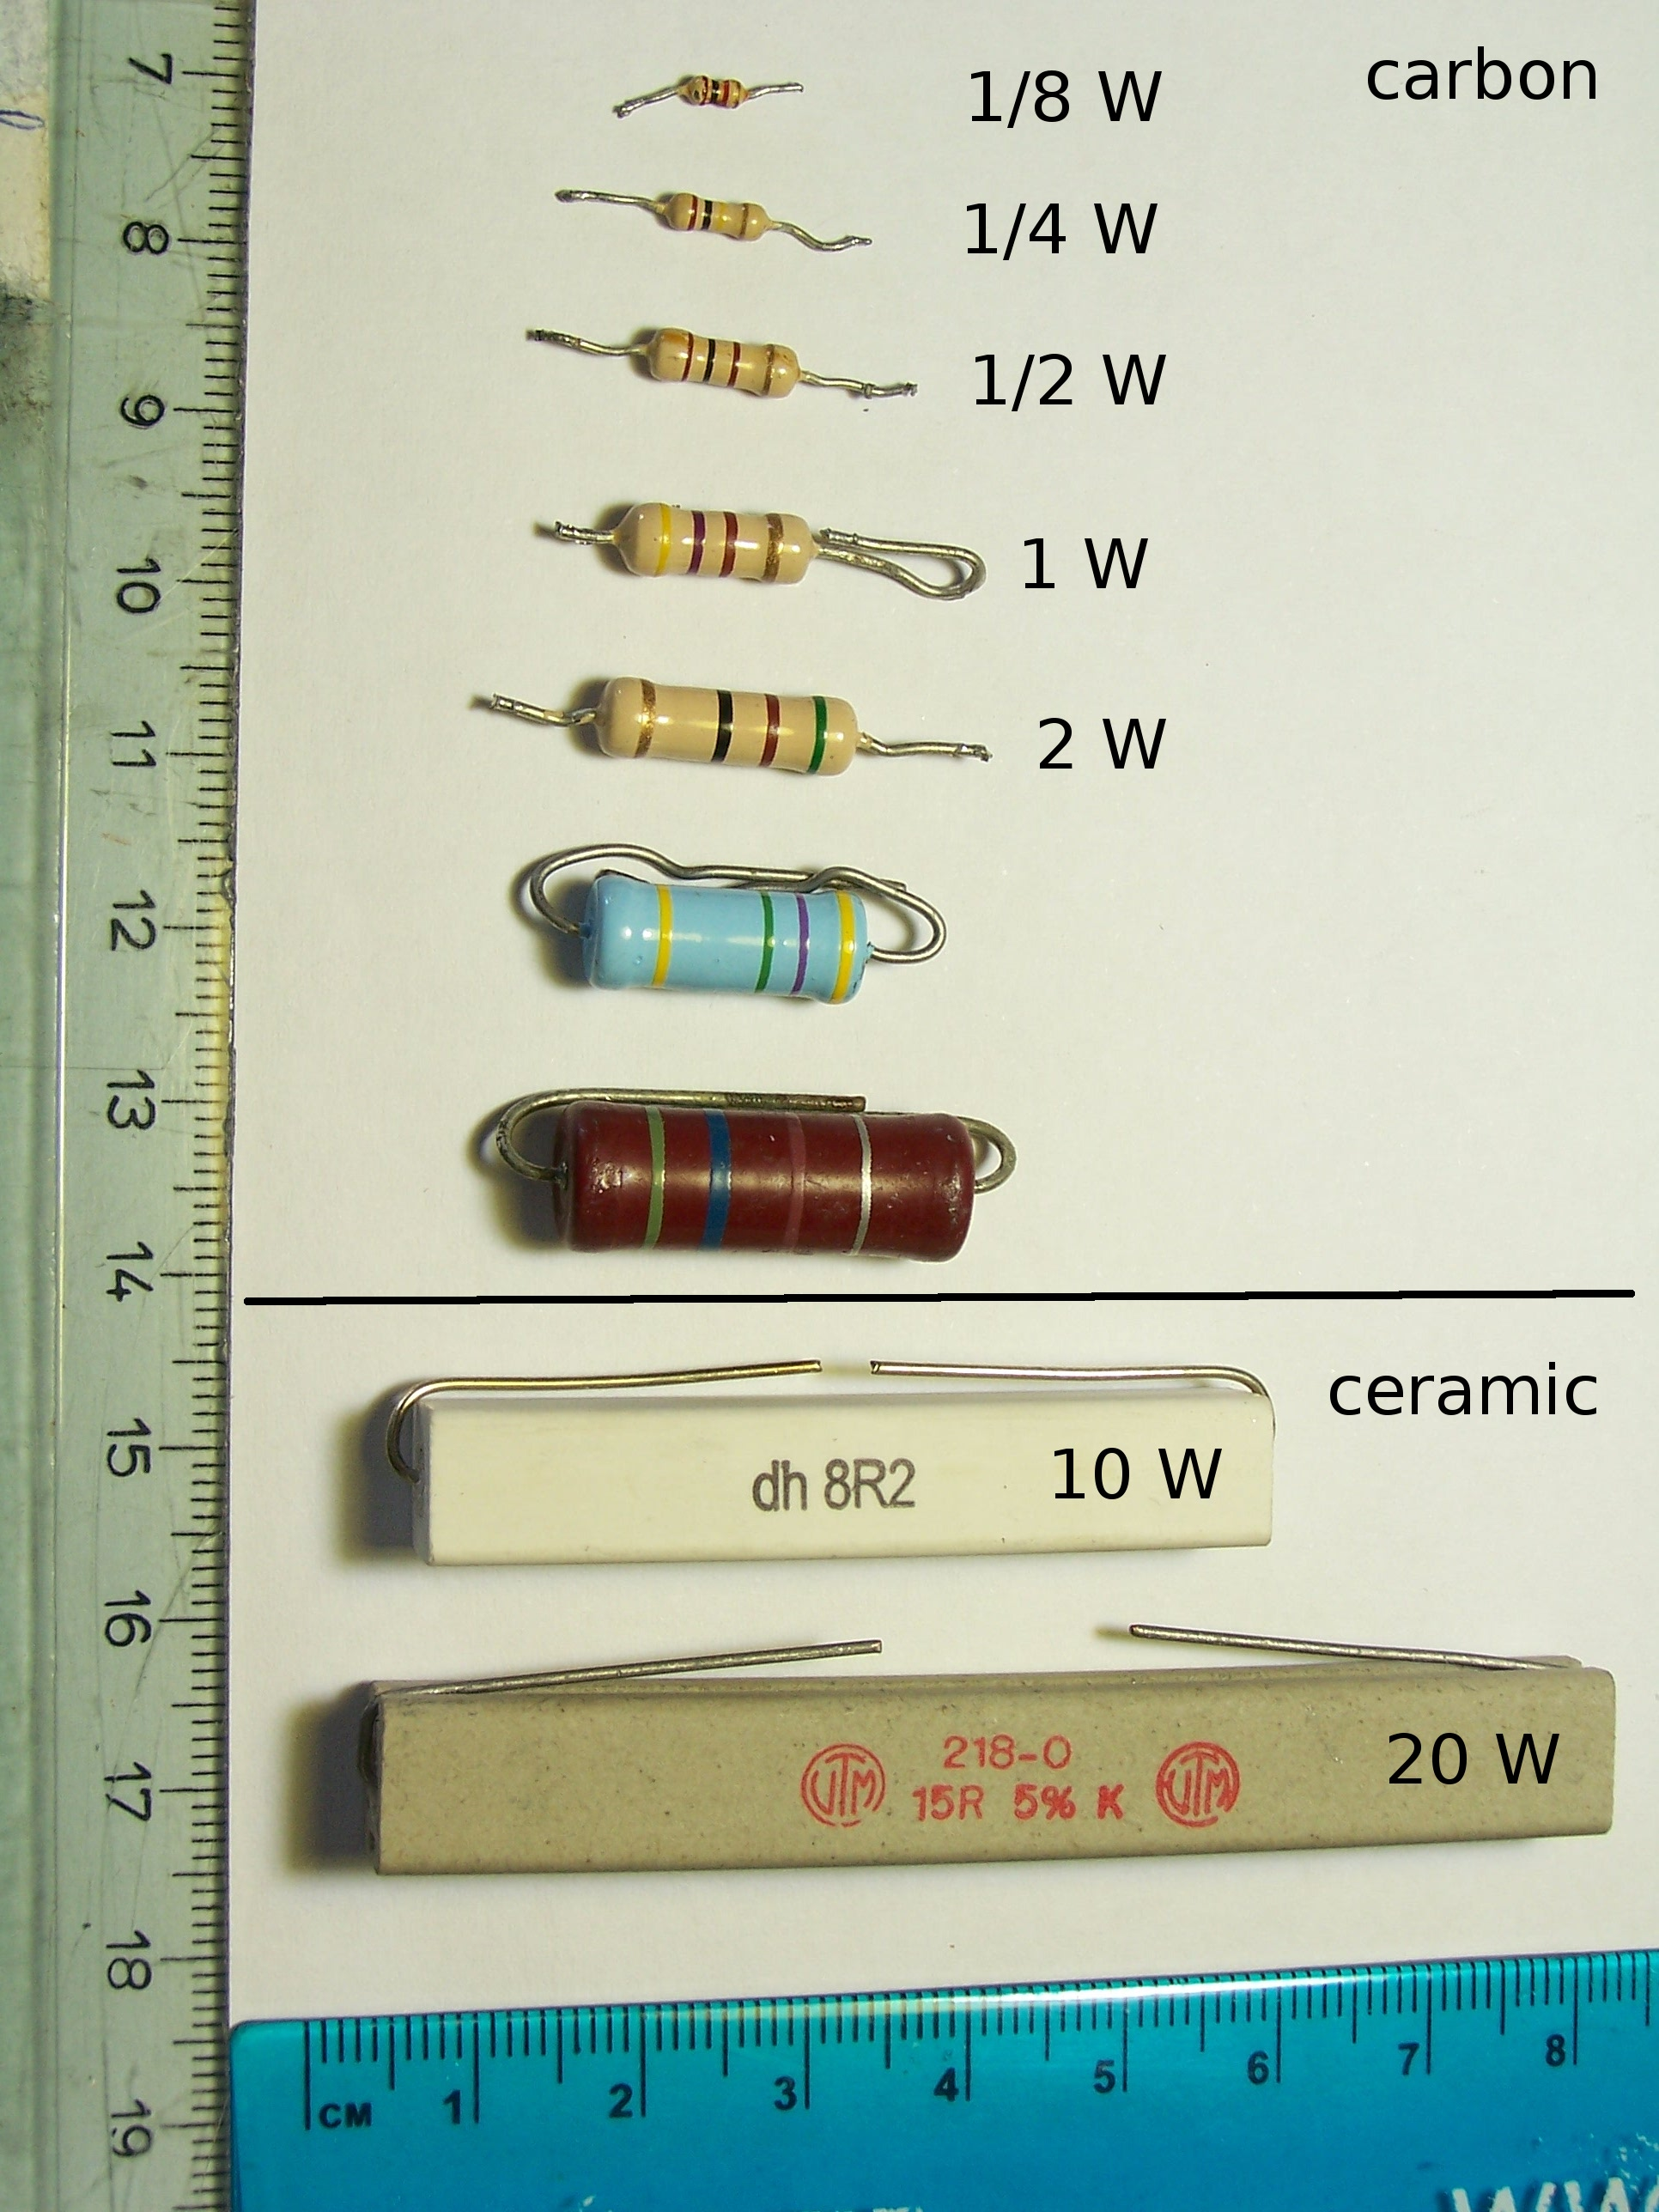
\includegraphics[width=0.35\textwidth]{laborator_01/figuri/7_resistors_power_ratings}
	\caption{Rezistoare -- puteri maxim admise \cite{rezistoare_puteri}.}
	\label{fig:rezistoare_puteri}
\end{figure}

Rela'tia \ref{eq:sarcina} arat'a c'a tensiunea de ie'sire nu este afectat'a de sarcin'a dac'a rezisten'ta de sarcin'a $R_s$ este mult mai mare decat $R_2$, sau altfel spus, dac'a $R_2 \ll R_s$. Dac'a $R_s$ este impus'a 'si cunoscut'a, atunci e indicat s'a alegem $R_2$ ('si implicit $R_1$ 'in func'tie de raportul $\alpha$ dorit) c\^at mai mic'a. 
%raportat'a la rezisten'ta de sarcin'a (de exemplu de 100 de ori mai mic'a).

\begin{retine}
Valori mici ale rezisten'telor $R_1$ 'si $R_2$ cresc precizia circuitului divizor de tensiune.
\end{retine}

Pe de alt'a parte, cu c\^at alegem rezisten'tele $R_1$ 'si $R_2$ mai mici, cu at\^at curentul care le str'abate este mai mare. Asta 'inseamn'a c'a puterea consumat'a de c'atre rezisten'te $P = RI^2$ va fi mai mare, deci ele se vor 'inc'alzi mai mult 'si se pot distruge. Dimensiunea rezistoarelor arat'a maximul de putere care e disipat'a 'inainte ca temperatura s'a creasc'a excesiv de mult (Fig. \ref{fig:rezistoare_puteri}).

\begin{retine}
Valori mari ale rezisten'telor $R_1$ 'si $R_2$ scad curentul deci 'si puterea consumat'a.
\end{retine}

\begin{exercise}
Determina'ti curentul maxim care poate str'abate un rezistor cu rezisten'ta de $180~\Omega$ 'si o putere maxim'a admis'a de 0.25 W. 
\end{exercise}

'In alegerea valorilor rezisten'telor trebuie c'autat echilibrul 'intre precizie 'si putere consumat'a. 

\begin{exercise}
Proiecta'ti un divizor de tensiune cu 4, care va fi alimentat cu o tensiune de $8$ V, conform Fig. \ref{fig:7_exercitiul1}. Rezisten'tele folosite au o putere maxim'a admis'a de $0.25$ W.
\end{exercise}

\begin{figure}[!t]
	\centering
		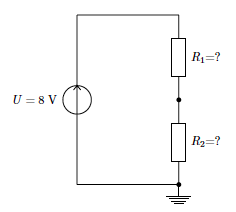
\includegraphics[width=0.5\textwidth]{laborator_01/figuri/7_exercitiul1}
	\caption{Proiectarea unui divizor de tensiune cu 4. Rezisten'tele au o putere maxim'a admis'a de 0.25 W.}
	\label{fig:7_exercitiul1}
\end{figure}
\section{Preg'atirea 'si notarea laboratorului}

%Nota la acest laborator va fi format'a dup'a cum urmeaz'a:

%\subsection*{'Inainte de lucrarea practic'a: 40\%}
\subsection*{'Inainte de lucrarea practic'a: recomandare}

F'ar'a o pregatire prealabil'a a laboratorului, nu ve'ti avea timp s'a termina'ti lucrarea practic'a. De aceea v'a recomand'am urm'atoarele:

\begin{itemize}
\item[--] Citi'ti cu aten'tie sec'tiunile \thechapter.1, \thechapter.2, \thechapter.3 ale acestei lucr'ari.
\item[--] Rezolva'ti cele dou'a chestionare de antrenament de pe moodle p\^an'a 'in preziua laboratorului.
\item[--] Pentru bonus. Rezolva'ti exerci'tiile scriind r'aspunsuri pe foi, preg\^atind foi de calcul \textit{.xls}, circuite (\textit{.cir} sau \textit{.asc}). Prinde'ti toate aceste foi 'intr-un dosar de laborator.
\end{itemize}

%Studen'tii vor completa chestionarul preliminar ''Stiu deja'' (QUIZ 1) pe moodle, care con'tine no'tiuni introductive de teorie, poate fi rulat de oric\^ate ori 'si se inchide cu o zi 'inainte de laborator.
%
%Dup'a citirea conceptelor din acest document, studen'tii vor completa chestionarul preliminar ''Am 'in'teles'' (QUIZ 2) pe moodle, care verific'a 'in'telegerea conceptelir prezentate 'in lucrare, poate fi rulat de oric\^ate ori 'si se inchide cu o zi 'inainte de laborator.
%
%Studen'tii vor aduce un draft de referat de laborator (pe hartie 'si foi imprimate ale fi'selor de calcul/fi'sierelor Spice) care va con'tine rezolvarea exerci'tiilor din capitolul de Concepte 'si cel de Simul'ari.

\subsection*{'In timpul lucr'arii practice: 100\%}
Acest punctaj va fi acordat 'in urma experimentelor 'si complet'arii celui de-al treilea chestionar, 'in timpul laboratorului.

\subsection*{Dup'a lucrarea practic'a: pentru bonus}
Completa'ti un referat de laborator cu rezultatele experimentelor 'si concluzii personale. Documentul va fi scris de m\^an'a 'si va con'tine foi imprimate acolo unde este cazul. Referatul trebuie s'a aib'a un cuprins coerent, de exemplu:

\begin{enumerate}
\item Introducere
\item Rezolvarea exerci'tiilor 
\item Rezultate experimentale
\item Concluzii personale
\end{enumerate}


%
%\begin{theorem}[Logic algebra]
%  \label{th:logicalgebra}
%  \index{logic algebra}
%  Let $P$, $Q$ and $R$ be logical propositions (true or false).
%  Then the following propositions are true:
%  \small
%  \begin{align*}
%    P \land Q &\Leftrightarrow Q \land P &
%    P \lor  Q &\Leftrightarrow Q \lor P  &&
%    \text{(commutative laws)} \\
%    (P \land Q) \land R &\Leftrightarrow P \land (Q \land R) &
%    (P \lor Q)  \lor  R &\Leftrightarrow P \lor  (Q \lor  R) &&
%    \text{(associative laws)} \\
%    P \land (Q \lor  R) &\Leftrightarrow (P \land Q) \lor  (P \land R) &
%    P \lor  (Q \land R) &\Leftrightarrow (P \lor  Q) \land (P \lor  R) &&
%    \text{(distributive laws)} \\
%    \lnot (P \land Q) &\Leftrightarrow \lnot P \lor  \lnot Q &
%    \lnot (P \lor  Q) &\Leftrightarrow \lnot P \land \lnot Q &&
%    \text{(De Morgan's laws)}
%  \end{align*}
%\end{theorem}
%\begin{proof}
%  \newcommand{\T}{\mathsf{T}}
%  \newcommand{\TT}{\mathbf{T}}
%  \renewcommand{\F}{\mathsf{F}}
%  We prove the first of De Morgan's laws and leave the proofs of
%  the remaining propositions as exercises. To prove the statement,
%  we create a truth table and fill in all possible values (true or
%  false) for the propositions $P$ and $Q$. Each of these propositions
%  can be either true or false and we thus obtain the following truth
%  table with four cases:
%  \begin{center}
%    \begin{tabular}{cccccccccc}
%      $\lnot$ & ($P$ & $\land$ & $Q$) & $\Leftrightarrow$ & $\lnot$ & $P$ & $\lor$ & $\lnot$ & $Q$ \\
%      \midrule
%      & $\T$ && $\T$ &&& $\T$ &&& $\T$ \\
%      & $\T$ && $\F$ &&& $\T$ &&& $\F$ \\
%      & $\F$ && $\T$ &&& $\F$ &&& $\T$ \\
%      & $\F$ && $\F$ &&& $\F$ &&& $\F$
%    \end{tabular}
%  \end{center}
%  By definition of the logical operators, we compete the table to obtain
%  \begin{center}
%    \begin{tabular}{cccccccccc}
%      $\lnot$ & ($P$ & $\land$ & $Q$) & $\Leftrightarrow$ & $\lnot$ & $P$ & $\lor$ & $\lnot$ & $Q$ \\
%      \midrule
%      $\F$ & $\T$ & $\T$ & $\T$ & $\TT$ & $\F$ & $\T$ & $\F$ & $\F$& $\T$ \\
%      $\T$ & $\T$ & $\F$ & $\F$ & $\TT$ & $\F$ & $\T$ & $\T$ & $\T$& $\F$ \\
%      $\T$ & $\F$ & $\F$ & $\T$ & $\TT$ & $\T$ & $\F$ & $\T$ & $\F$& $\T$ \\
%      $\T$ & $\F$ & $\F$ & $\F$ & $\TT$ & $\T$ & $\F$ & $\T$ & $\T$& $\F$
%    \end{tabular}
%  \end{center}
%  It follows that the statement we want to prove (the equivalence $\Leftrightarrow$)
%  is always true (a \emph{tautology}), which proves the statement.
%\end{proof}


%\begin{definition}[Rational Cauchy sequence]
%  \label{th:rationalcauchysequence}
%  \index{rational Cauchy sequence}
%  A rational Cauchy sequence is a rational sequence
%  $(x_n)_{n=0}^{\infty}$ such that
%  \begin{equation}
%    \forall \epsilon \in \mathbb{Q}_+ \;
%    \exists N \in \mathbb{N} : m, n \geq N \Rightarrow |x_m - x_n| < \epsilon.
%  \end{equation}
%  In other words, for each (small) rational number $\epsilon > 0$
%  there is a (big) number $N$ such that the distance $|x_m - x_n|$
%  between $x_m$ and $x_n$ is less than $\epsilon$ if both $m$ and $n$
%  are larger than or equal to $N$.
%\end{definition}
%
%\begin{remark}
%  A remark may be in order here. This definition is concerned with
%  \emph{rational} Cauchy sequences. We will later encounter a similar
%  definition of \emph{real} Cauchy sequences.
%\end{remark}
%
%\begin{example}[Solving the equation $x^2 = 2$]
%  Consider the equation $x^2 = 2$. It is easy to prove that this
%  equation does not have any rational solutions. However, consider
%  the following iteration formula:
%  \begin{equation}
%    x_n = \frac{x_{n-1} + 2 / x_{n - 1}}{2},
%  \end{equation}
%  where $n = 1,2,3,\ldots$ and $x_0 = 1$. The resulting sequence of
%  rational numbers quickly approaches a number in the vicinity of
%  $x = 1.4142135623731$:
%  \begin{displaymath}
%    \begin{array}{rclcl}
%      x_0 &=& 1 \\
%      x_{1} &=& (x_{0} + 2 / x_{0}) / 2 &=& 1.5 \\
%      x_{2} &=& (x_{1} + 2 / x_{1}) / 2 &\approx& 1.4166666666667 \\
%      x_{3} &=& (x_{2} + 2 / x_{2}) / 2 &\approx& 1.4142156862745 \\
%      x_{4} &=& (x_{3} + 2 / x_{3}) / 2 &\approx& 1.4142135623747 \\
%      x_{5} &=& (x_{4} + 2 / x_{4}) / 2 &\approx& 1.4142135623731 \\
%      x_{6} &=& (x_{5} + 2 / x_{5}) / 2 &\approx& 1.4142135623731 \\
%      x_{7} &=& (x_{6} + 2 / x_{6}) / 2 &\approx& 1.4142135623731 \\
%      x_{8} &=& (x_{7} + 2 / x_{7}) / 2 &\approx& 1.4142135623731 \\
%      x_{9} &=& (x_{8} + 2 / x_{8}) / 2 &\approx& 1.4142135623731 \\
%      x_{10} &=& (x_{9} + 2 / x_{9}) / 2 &\approx& 1.4142135623731
%    \end{array}
%  \end{displaymath}
%  We will later see that this iteration, or any other equivalent
%  iteration, defines the real number $\sqrt{2}$.
%\end{example}

%\section{Third section}
%
%Now let's move on to the definition of the real number system. This
%may be defined in a multitude of ways, one of which is to think about
%a real number as a rational Cauchy sequence, or rather the equivalence
%class of Cauchy sequences ``converging to'' that number.
%
%\begin{definition}[The real numbers $\mathbb{R}$]
%  \label{def:realnumbers}
%  \index{real numbers}
%  The real numbers $\mathbb{R}$ is the set of all equivalence classes
%  of rational Cauchy sequences.
%\end{definition}
%
%Now that this is settled, lets prove the completeness of the real
%number system.
%
%\begin{theorem}[The completeness of the real numbers]
%  \label{th:realnumberscomplete}
%  \index{completeness of the real numbers}
%  Let $(x_n)_{n=0}^{\infty}$ be a sequence of real numbers.
%  Then $(x_n)_{n=0}^{\infty}$ is convergent if and only if
%  it is also a real Cauchy sequence.
%  \end{theorem}
%\begin{proof}
%  Write $x_m = [(x_{mn})_{n=0}^{\infty}]$ where
%  $x_{mn}$ is the $n$th number in a rational Cauchy sequence
%  representing the real number $x_m$. And so on\ldots.
%\end{proof}
%
%For further reading, there are several excellent works that one could
%cite, such as \cite{Tao2006,Turing1936}.
%
%\section*{Exercises}
%
%\begin{exercise}
%  Let $A = \{1, 2, 3\}$ and $B = \{2, 3, 4\}$.
%  Determine the following sets. \\
%  (a) $A \cup B$ \quad
%  (b) $A \cap B$ \quad
%  (c) $A \setminus B$ \quad
%  (d) $A \times B$
%\end{exercise}
%
%\begin{exercise}
%  Let $A = \{1, 3, 5, 7, 9\}$ and $B = \{2, 4, 6, 8, 10\}$.
%  Determine the following sets. \\
%  (a) $A \cup B$ \quad
%  (b) $A \cap B$ \quad
%  (c) $A \setminus B$ \quad
%  (d) $A \times B$
%\end{exercise}
%
%\begin{exercise}
%  Let $A = \{1, 2, 3\}$, $B = \{2, 3, 4\}$ and $C = \{3, 4, 5\}$.
%  Determine the following sets. \\
%  (a) $A \cup B \cup C$ \quad
%  (b) $A \cap B \cap C$ \quad
%  (c) $(B \setminus A) \cap C$ \quad
%  (d) $(A \times B) \times C$
%\end{exercise}
%
%\section*{Problem}
%
%\begin{problem}
%  Interpret the following set definition (Russell's paradox) and discuss
%  whether $X \in X$ or $X \notin X$:
%  \begin{equation}
%    X = \{x \mid x \notin x\}.
%  \end{equation}
%\end{problem}
%
%\section*{Computer exercises}
%
%\begin{programming}
%  Write a program that generates the sequence $(x_n)_{n=0}^{100}$
%  for $x_n = n$.
%\end{programming}
%
%\begin{programming}
%  Write a program that generates the odd numbers between $1$ and $100$.
%\end{programming}
%
%\begin{programming}
%  Write a program that computes the sum $\sum_{n=0}^{100} x_n$
%  for $x_n = n$.
%\end{programming}

%---------------------------------------------------------------------------
%\chapter{Second chapter}
%
%\begin{summary}
%  \blindtext
%\end{summary}
%
%\section{First section}
%\Blindtext
%
%\section{Second section}
%\Blindtext
%
%\section{Third section}
%\Blindtext
%
%%---------------------------------------------------------------------------
%\chapter{Third chapter}
%
%\begin{summary}
%  \blindtext
%\end{summary}
%
%\section{First section}
%\Blindtext
%
%\section{Second section}
%\Blindtext
%
%\section{Third section}
%\Blindtext

%---------------------------------------------------------------------------
% Bibliography
%---------------------------------------------------------------------------

\addcontentsline{toc}{chapter}{\textcolor{tssteelblue}{Referin'te}}
\printbibliography[title = Referin'te]{}

%---------------------------------------------------------------------------
% Index
%---------------------------------------------------------------------------

\printindex

\end{document}
